\documentclass[14pt, a4paper]{extarticle}
% Русская локализация
\usepackage[english,russian]{babel}


\usepackage{appendix}
\usepackage{alphabeta}

% Использование математических шрифтов
\usepackage{unicode-math}

% Шрифты
\usepackage{fontspec}
\usepackage{courier}
\defaultfontfeatures{Ligatures={TeX},Renderer=Basic}
\setmainfont[Ligatures={TeX}]{Times New Roman}
\setmonofont{Courier New}
\setmathfont{XITS Math}

% Расширенные ссылки
\usepackage{nameref}

% Оформление URL
\usepackage{xurl}
\usepackage{hyperref}
\hypersetup{
  colorlinks,
  citecolor=black,
  filecolor=black,
  linkcolor=black,
  urlcolor=black,
  breaklinks=true,
}
\urlstyle{same}

% Поддержка изображений
\usepackage{graphicx}
\graphicspath{{./images/}}
\DeclareGraphicsExtensions{.jpg,.png}
\usepackage{svg}

% Таблицы
\usepackage{tabularx}
\usepackage{tabulary}
\usepackage{ltablex}
\usepackage{multirow}
\usepackage{hhline}
% Выравнивание по левому краю, с многострочностью
\newcolumntype{s}{>{\raggedright\arraybackslash}X}

% Поддержка листингов
\usepackage{listings}
\lstdefinestyle{gost}{
  basicstyle=\ttfamily\footnotesize,
  breakatwhitespace=false,
  breaklines=true,
  keepspaces=true,
  showspaces=false,
  showstringspaces=false,
  frame=single
}
\lstset{style=gost}%

% Отступ первой строки первого абзаца
\usepackage{indentfirst}
\linespread{1.25}

% Размер полей в документе
\usepackage{geometry}
\geometry{left=3cm}
\geometry{right=1cm}
\geometry{top=2cm}
\geometry{bottom=2cm}

% Абзацный отступ
\setlength{\parindent}{1.25cm}

% Отступ для элементов в списке
\usepackage{enumitem}
\setlist{left=\parindent, labelsep=1cm, itemsep=0pt, topsep=0pt}

% Загрузка pdf-документов (нужно для титульных листов)
\usepackage[final]{pdfpages}
% Возможность поворота pdf файло
\usepackage{pdflscape}
\usepackage{everypage}

\newcommand{\Lpagenumber}{\ifdim\textwidth=\linewidth\else\bgroup%
    \dimendef\margin=0 %use \margin instead of \dimen0
    \ifodd\value{page}\margin=\oddsidemargin
    \else\margin=\evensidemargin%
    \fi

\raisebox{\dimexpr-\topmargin-\headheight-\headsep-0.5\linewidth}[0pt][0pt]{%
      \rlap{\hspace{\dimexpr-\margin+\textheight+\footskip}%
        \llap{\rotatebox{90}{\thepage}}}}%
    \egroup\fi}
\AddEverypageHook{\Lpagenumber}%

\usepackage{float}
% Форматирование подписей
\usepackage{caption}

\usepackage{newfloat}
% \DeclareCaptionType{listing}

\DeclareCaptionLabelSeparator{emdash}{\;\textemdash\;}
\captionsetup[figure]{name={Рисунок}, labelsep=emdash, justification=centering,
position=above, singlelinecheck=off, font={small, bf}, labelfont=bf, skip=6pt}
\captionsetup[table]{name={Таблица}, labelsep=emdash,
justification=raggedright, position=top, singlelinecheck=off, font={small, it},
labelfont=it, skip=6pt, margin=0cm}
% \captionsetup[lstlisting]{labelsep=emdash, justification=raggedright,
% position=top, singlelinecheck=off, font={small, it}, labelfont=it, skip=6pt,
% margin=0cm}

% Нумеровать внутри заголовков первого уровня
\counterwithin{figure}{section}
\counterwithin{table}{section}
% \counterwithin{lstlisting}{section}
\AtBeginDocument{\counterwithin{lstlisting}{section}}

% Отключение переносов текста
\usepackage{ragged2e}
\justifying
\tolerance=500
\hyphenpenalty=10000
\emergencystretch=3em

% Форматирование заголовков
\usepackage{titlesec}
% Оформление заголовка первого уровня
% Полужирное начертание
% Кегль 18 пт
% С новой страницы
\titleformat{\section}[block]
{\newpage\bfseries\fontsize{18pt}{21.6pt}\selectfont}
{\thesection}
{1em}{}
% Оформление ненумерованных заголовков (Введение, Содержание, список
% источников, и.т.д.)
\titleformat{name=\section,numberless}[block]
{\centering\newpage\bfseries\fontsize{18pt}{21.6pt}\selectfont}
{}
{0em}{}{}
% Отступы у заголовков первого уровня
\titlespacing{\section}
{\parindent}% отступ слева (равен 1.25 см, как у отступа первой строки абзаца)
{0em}% интервал перед
{10mm}% интервал после
% Оформление заголовков второго уровня
\titleformat{\subsection}[block]
{\bfseries\fontsize{16pt}{19.2pt}\selectfont}
{\thesubsection}
{1em}{}
% Отступы у заголовков второго уровня
\titlespacing{\subsection}
{\parindent}% пробел слева
{15mm}% отступ перед
{10mm}% отступ после
% Оформление заголовков второго уровня
\titleformat{\subsubsection}[block]
{\bfseries\selectfont}
{\thesubsection}
{1em}{}
% Отступы у заголовков второго уровня
\titlespacing{\subsubsection}
{\parindent}% пробел слева
{15mm}% отступ перед
{10mm}% отступ после


% Оформление заголовков в содержании
\usepackage{titletoc}
\contentsmargin{0pt}
\renewcommand\contentspage{\thecontentspage}
\dottedcontents{section}[2.3em]{}{2.3em}{5pt}
\dottedcontents{subsection}[2.3em]{}{2.3em}{5pt}
% Оформление приложений
\usepackage{appendix}
\renewcommand\appendixpagename{ПРИЛОЖЕНИЯ}

% Подключение biblatex, с использованием стиля gost-numeric
\usepackage[
citestyle=gost-numeric,
style=gost-numeric,
blockpunct=emdash,
backend=biber,
sorting=none
]{biblatex}
% Запрет разрыва url ссылок
\defcounter{biburlnumpenalty}{3000}
\defcounter{biburlucpenalty}{6000}
\defcounter{biburllcpenalty}{9000}
% Добавление полей для ссылок и даты обращения к ним
\DeclareFieldFormat{url}{Режим доступа: #1}
\DeclareFieldFormat{urldate}{(Дата обращения: #1)}
\renewcommand*{\entrysetpunct}{\par\nopunct\!\!}
% Использовать prac.bib как источник
\addbibresource{diploma.bib}
% Форматирование заголовка библиографии
\defbibheading{bibliography}[\bibname]{%
  \section*{\centering #1}%
  \markboth{#1}{#1}}
  
\usepackage{etoolbox}
\AtBeginEnvironment{tabularx}{\fontsize{12pt}{14pt}\selectfont}


\usepackage{lipsum}
\usepackage{csquotes}

\begin{document}
\def\contentsname{СОДЕРЖАНИЕ}

% Загрузка титула
\pagenumbering{gobble}
\begin{titlepage}
  
\includepdf{title}
  
\includepdf[pages={1-5}]{title}
\end{titlepage}
\pagenumbering{arabic}
\setcounter{page}{7}
% Содержание
\tableofcontents

\section*{ГЛОССАРИЙ}
\phantomsection
\addcontentsline{toc}{section}{ГЛОССАРИЙ}
\begin{raggedright}
  VPC --- Virtual Private Cloud (виртуальная частная сеть). \\
  ЦОД --- Центр обработки данных. \\
  СХД --- Система хранения данных. \\
  СПО --- Системное программное обеспечение. \\
  FC --- Fiber Channel (оптоволоконный канал). \\
  ИТ --- Информационные технологии. \\
  ИТ-инфраструктура --- Информационно-технологическая инфраструктура. \\
  CRM --- Управление взаимоотношениями с клиентами (Customer Relationship Management) \\
  СУБД --- Система управления базами данных \\
  ПО --- Программное обеспечение \\
  ОКВЭД --- Общероссийский классификатор видов экономической деятельности \\
  BPMN --- Нотация и модель бизнес-процессов (Business Process Model and Notation) \\
  SLA --- Соглашение об уровне предоставления услуги (Service Level Agreement) \\
  UML --- Унифицированный язык моделирования (Unified Modeling Language) \\
  DFD --- Диаграмма потоков данных (Data Flow Diagrams) \\
  CPU --- Центральный процессор (Central Processing Unit)\\
  CMS --- Система управления содержимым (Content management system) \\
  ФЗ --- Федеральный Закон\\
  PaaS ---  Платформа как услуга (Platform as a Service)\\
  SaaS --- ПО как услуга (Software as a Service)\\
  HA - Высокая доступность (High Availability)\\
\end{raggedright}

\section*{ВВЕДЕНИЕ}
\phantomsection
\addcontentsline{toc}{section}{ВВЕДЕНИЕ}

Исследуемым объектом в рамках проекта является сервис хранения и обработки
данных информационной системы модуля потребительского кредитования. Этот модуль включает в
себя ответственность за управление ипотечными и кредитными продуктами, так же
за хранение и обработку данных клиентов и генерацию отчетов, как по клиентам
так и работе модуля.

Актуальность темы исследования обусловлена стремительным развитием информационных
технологий и их внедрением во все сферы социально-экономической жизни, включая сектор
финансовых технологий. Кредитные организации в настоящее время находятся в условиях
сильной конкуренции, а это вынуждает активно внедрять новые технологии, в частности
цифровые технологии, которые позволяют оптимизировать затраты и внутренние процессы,
повышать качество обслуживания клиентов и обеспечивать устойчивость бизнес-моделеи.
В этом ключе важное значение приобретает проектирование и фунциольное моделирование
ИТ-инфраструктуры одного из ключевых элементов, который обеспечивает эффективаность
функционирования автоматизированных кредитных систем, а именно модуля потребительского
кредитования.

В отечественной и зарубежной литературе существует много работ, рассматриващих
проблемы проектирования и моделирования ИТ-инфраструктуры в которых так же
рассматриваются архитектурные подходы, выбор технических решений и методы оптимизации
процессов. Однако в условиях быстро меняющейся регуляторной и потребительской среды
задача создания адаптированной, масштабируемой и безопасной ИТ-инфраструктуры с учетом
специфики бизнес-процессов конкретной организации остается актуальной.

Целью данной работы является проектирование и функциональное моделирование
ИТ-инфраструктуры, поддерживающей модуль потребительского кредитования в
кредитной организации, включающего описание архитектуры и обоснование выбранного
программно-аппаратного решения.

Для достижения поставленной цели в работе решаются следующие задачи:

\begin{enumerate}
  \item Анализ вариантов поставки информационно-технологического сервиса;
  \item Анализ вариантов компонентов ИТ-инфраструктуры и обоснование выбранного варианта;
  \item Выбор системного программного обеспечения;
  \item Моделирование топологии развертывания;
  \item Составление спецификации рабочих станций;
  \item Моделирование топологии развертывания инструментального программного обеспечения;
  \item Анализ сетевой инфраструктуры и моделирование сетевой топологии.
\end{enumerate}

Практическая значимость работы заключается в возможности использования представленных
разработок для модернизации или внедрения модулей автоматизированных систем
потребительского кредитования в ИТ-инфраструктуру кредитных организаций, что
способствует повышению надежности, безопасности, отказоустойчивости и производительности.

\section{ПРОИЗВОДСТВЕННАЯ ПРАКТИКА}

\subsection{Анализ вариатнов поставки информационно-технологического сервиса}

В работе произведен анализ четырех вариантов поставки
информационно-технологического сервиса, который включает в себя выбор между
такими вариантами поставки, как полностью самостоятельный, облачный (SaaS, Paas, IaaS),
мульти-облачный и гибридный. На основе анализа выбран, как самый оптимальный вариант
поставки, полностью самостоятельный вариант.

Полностью облачный сервис \cite{micrasoft-azure-book} по одному из моделей SaaS,
PaaS или IaaS, позволяет снизить затраты на содержание и поддержку ИТ-инфраструктуры,
но не является лучшим решением, так как вводит за собой ряд ограничений, таких как
сильная зависимость от поставщика, ограниченные возможности кастомизации и настройки,
а также, что является критичным, возможные проблемы с безопасностью и сохранностью данных.

Мульти-облачный вариант, подразумевает под собой так же использование облачной
инфраструктуры, но в отличие от полностью облачного варианта, позволяет использовать
разные облачные решения от разных поставщиков, что позволяет избежать
некоторых проблем, связанных с безопасностью и кастомизацией. Однако, данный
вариант так же не является оптимальным, так как требует высококвалифицированных
специалистов для поддержки и настройки, а так же имеет риски конфликтов совместимости,
что существенно сказывается на затратах.

Гибридный подход позволяет совместное исопльзование облачных решений и собственных
ресурсов. Такой вариант позволяет наиболее гибко и без особых затруднений масштабировать
инфраструктуру, но является более дорогим в долгосрочной перспективе, не исключает
пенно данный подход является наиболее гибким, чтобы отвечать всем требованиям
регуляторов и требованиям хранения персональных данных, например, Федеральный закона
№152-ФЗ <<О персональных данных>>.

Полностью самостоятельный вариант поставки инфраструктуры предполагает использование собственных серверов, систем хранения данных и сетевого оборудования, размещённых в арендованной серверной стойке в центре обработки данных (ЦОД). Такой подход обеспечивает полный контроль над данными и инфраструктурой, что особенно важно для соблюдения требований регуляторов, таких как Федеральный закон №152-ФЗ <<О персональных данных>>.

Основными преимуществами данного варианта являются полный контроль над чувствительными данными и инфраструктурой, отсутствие зависимости от облачных поставщиков, возможность гибкой настройки и масштабирования в соответствии с требованиями бизнеса, а также соответствие требованиям регуляторов и стандартов безопасности.

Однако данный подход также имеет свои недостатки. К ним относятся высокие первоначальные затраты на закупку оборудования и развертывание инфраструктуры, необходимость содержания квалифицированного ИТ-персонала для обслуживания и поддержки, а также более длительное время внедрения по сравнению с облачными решениями.

В Таблице\;\ref{tab:infra_options} приведено сравнение всех четырех вариантов поставки
инфраструктуры. Таблица позволяет точечно рассмотреть все возможные варианты, их
преимущества и недостатки.

\begin{tabularx}{\textwidth}{|l|X|X|}
  \caption{Сравнение вариантов поставки ИТ-инфраструктуры\label{tab:infra_options}} \\
  \hline
  Вариант поставки            & Преимущества & Недостатки                           \\\hline
  \endfirsthead
  \caption*{Продолжение таблицы~\ref{tab:infra_options}}                            \\
  \hline
  Вариант поставки            & Преимущества & Недостатки                           \\\hline
  \endhead
  \endfoot
  \endlastfoot

  Полностью самостоятельный   &
  Частный контроль над чувствительныи данными и инфраструктурой;
  отсутствие зависимости от облачных поставщиков;
  гибкость в соответствии требованиям регуляторов (например, 152-ФЗ).
                              &
  Высокие первоначальные затраты на развертывание;
  необходимость содержания ИТ-персонала;
  более длительное внедрение.                                                       \\\hline

  Облачный (SaaS, PaaS, IaaS) &
  Более низкие затраты на поддержку и обслуживание;
  быстрое масштабирование и внедрение;
  меньшая потребность в локальных ресурсах.
                              &
  Сильная зависимость от поставщика;
  ограниченные возможности настройки;
  риски утечки данных и проблемы с безопасностью.                                   \\\hline

  Мульти-облачный             &
  Снижение зависимости от одного поставщика;
  гибкость в выборе сервисов;
  потенциально лучшая безопасность.
                              &
  Необходимость высококвалифицированного персонала;
  риски несовместимости решений;
  повышенные затраты на администрирование;
  риски утечки данных и проблемы с безопасностью.                                   \\\hline

  Гибридный                   &
  Гибкость масштабирования;
  возможность совмещать преимущества облака и локальной инфраструктуры;
  частичный контроль над критичными компонентами.
                              &
  Более высокая стоимость в долгосрочной перспективе;
  повышенные затраты на администрирование;
  не исключены риски утечки данных; сложность интеграции компонентов.               \\\hline
\end{tabularx}

На основе описанных выше данных становится понятно, что для модуля потребительского кредитования
оптимальным вариантом является полностью самостоятельный вариант поставки, так как он позволяет
иметь полный контроль над данными и инфраструктурой, окупается в долгосрочной перспективе, не
требует высококвалифицированного персонала и позволяет избежать проблем с безопасностью.

Компоненты инфраструктуры размещены в серверной стойке внутри
Центра обработки данных (ЦОД) предоставляемым Selectel \cite{selectel-web}.
Selectel это Россйская компания, которая предоставляет услуги облачных вычислений,
выделенных серверов и услуги по размещению оборудования в ЦОД. Базовая тарификация
серверной стойки включает в себя 5 кВА мощности и 30ТБ интернет трафика в месяц.
Оба этих параметра предоставляются бесплатно при базовом тарифе, при необходимости
большей мощности, трафика или же 10ГБит/с портов, Selectel предоставляет возможность
доплатить. Вендор обеспечивает круглосуточную поддержку и мониторинг оборудования с
базовым удаленным обслуживаем.

Такой подход к размещению инфраструктуры позволяет избежать затрат на содержание,
позволяет избавиться от затрат на сетевое оборудование, так как вендор предоставляет
все необходимое оборудование и нужные каналы связи в аренду.

В связи с тем, что сохранность пользовательских данных является критически важной,
то в проектируемой инфраструктуре предусмотрено использование системы резервного,
которая заключается в полном дублировании данных СХД на облачное блочное хранилище
(Cold Object Storage) предоставляемое вендором Selectel \cite{selectel-block-storage}.
Объектное хранилище предоставляемое вендором по официальной документации полностью
соответствует требованиям регуляторов и федеральному закону №152-ФЗ <<О персональных
данных>>.

Структурная модель выбранного моделя поставки ИТ-инфраструктуры представлена на
Рисунке\;\ref{fig:infra1}.

\begin{figure}[H]
  \centering
  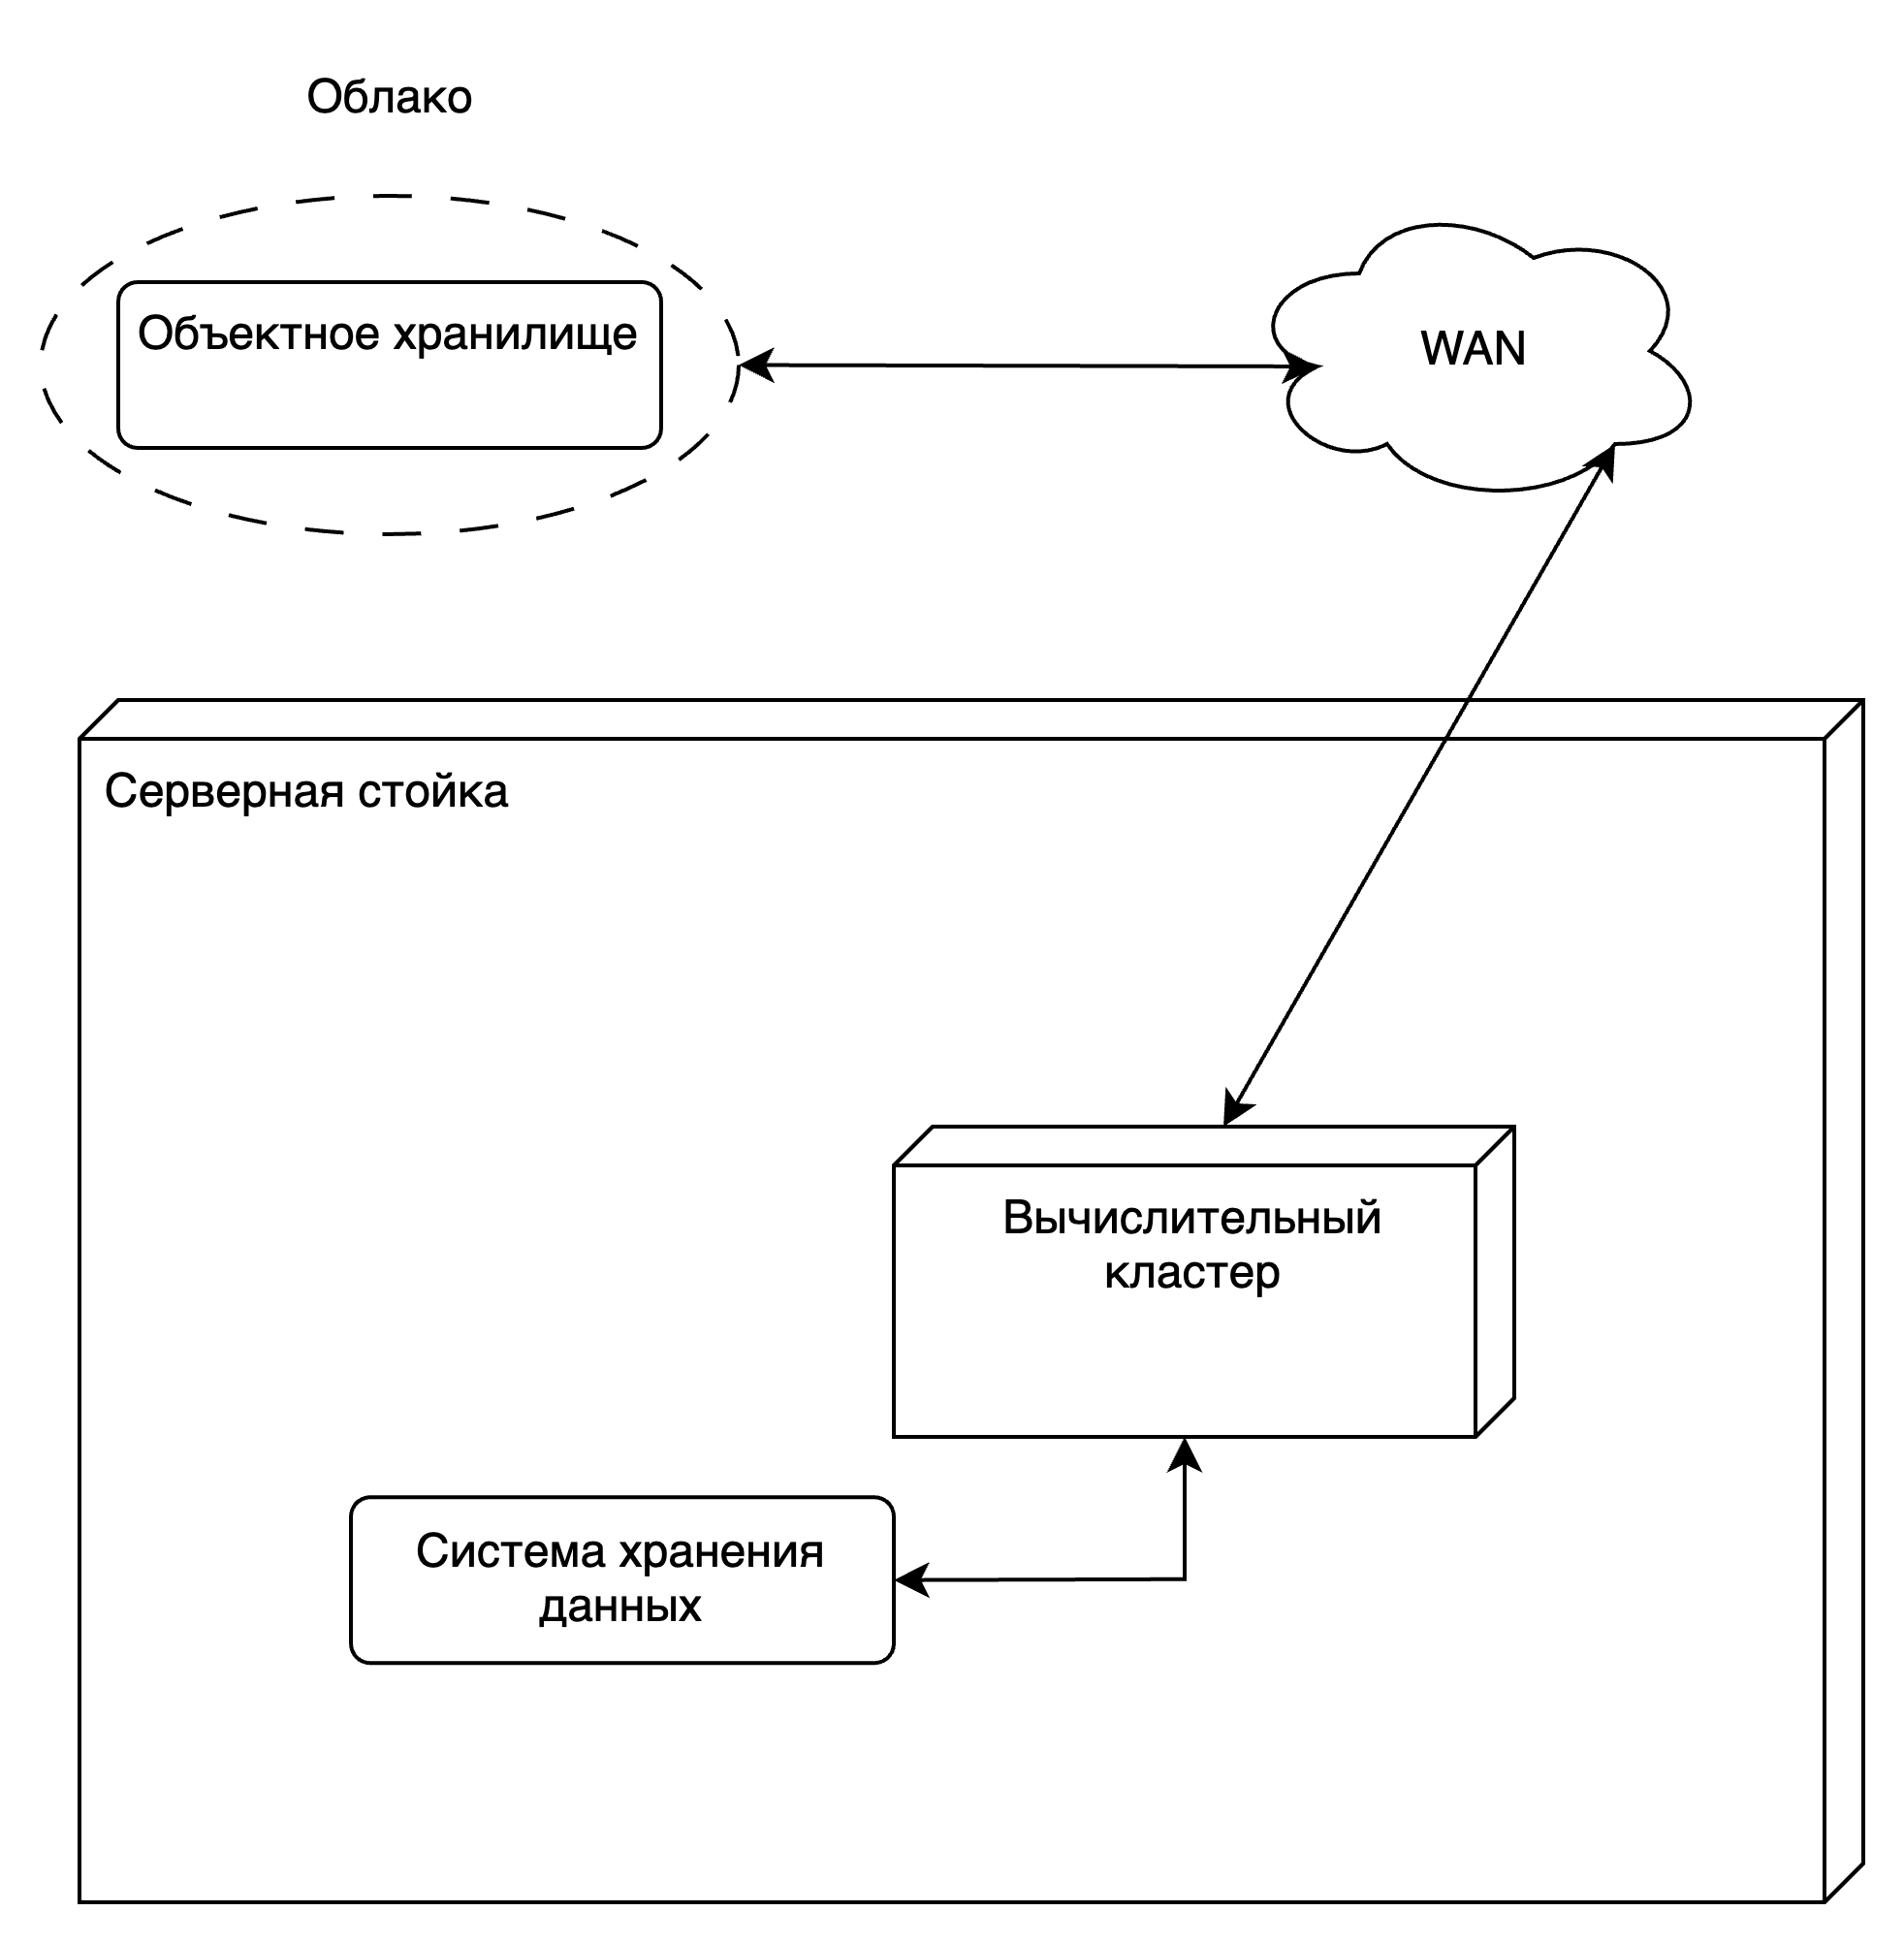
\includegraphics[width=0.6\textwidth]{infra1_3.png}
  \caption{Структурная модель выбранного моделя поставки ИТ-инфраструктуры}
  \label{fig:infra1}
\end{figure}

\subsection{Анализ вариантов компонентов ИТ-инфраструктуры}

В данном разделе произведен анализ возможных компонентов ИТ-инфраструктуры,
которые могут быть использованы в проектируемой инфраструктуре. Основными
компонентами являются серверы, системы хранения данных, сетевое оборудование,
системы резервного копирования и восстановления и системы виртуализации.

Основным критерием для инфраструктуры модуля потребительского кредитования
является отказоустойчивость, безопасность хранения данных и возможность
масштабирования. В связи с этим основные модули инфрастуктуры имеют дубликаты
физических компонентов.

Анализ серверов показывает, что для проектируемой инфраструктуры хорошим решением
является использование сервера средней мощности производителя присутствующего
в реестре минцифры РФ, что упрощает поиск и содержвание персонала для
обслуживания. Под указанные критерии подходит производитель оборудования <<Гравитон>> \cite{graviton-site}.
У произаводителя имеется широкий выбор серверов, которые поддерживают
разные конфигурации, наиболее подходящим является Сервер «Гравитон» С2122ИУ \cite{graiton-server-s2122iu}.
Данный эземпляр имеет большой потенциал для увеличения объема оперативной памяти,
в отличие от других серверов данной категории, поддерживает до двух процессоров Intel
Xeon. Поддерживает горячую замену блоков питания и вентиляторов, имеет встроенный
модуль управления BMC и полностью соответствует требованиям регуляторов.
Технические характеристики сервера приведены в Таблице\;\ref{tab:graviton_s2122iu}.

В сервер установлены два диска SSD SATA 2.5 типа <<Intel D3-S4610>> каждый на
1 ТБ для работоспособности гипервизора и работы системы.

Посколько сервер использует СХД для хранения данных, а подключение происходит
благодаря фабрике, это значит, что сервер требует установки дополнительного
контроллера HBA, так как изначально не имеет его. Установка контроллера
производится производителем по предзаказу самого сервера.

В сервер устанолено 2 процессора Intel Xeon Gold 6233 с тактовой частотой 2.5 ГГц,
он имеет 24 ядра и 48 потоков.

\begin{tabularx}{\textwidth}{|l|X|}
  \caption{Технические характеристики сервера Гравитон С2122ИУ\label{tab:graviton_s2122iu}}                                                                                                                \\
  \hline
  Параметр                             & Значение                                                                                                                                                          \\\hline
  \endfirsthead
  \caption*{Продолжение таблицы~\ref{tab:graviton_s2122iu}}                                                                                                                                                \\
  \hline
  Параметр                             & Значение                                                                                                                                                          \\\hline
  \endhead
  \endfoot
  \endlastfoot

  Процессор                            & До 2× Intel Xeon 4-го или 5-го поколения (TDP до 150 Вт)                                                                                                          \\\hline
  Сокет                                & 2× LGA 4677                                                                                                                                                       \\\hline
  Чипсет                               & Intel C741                                                                                                                                                        \\\hline
  Оперативная память                   & До 8 ТБ DDR5; 32 слота DIMM                                                                                                                                       \\\hline
  Поддерживаемые модули памяти         & RDIMM: 8/16/32/64 ГБ; LRDIMM: 64/128/256 ГБ                                                                                                                       \\\hline
  Форм-фактор                          & 2U, стойка 19"                                                                                                                                                    \\\hline
  Дисковая подсистема                  & Передняя панель: 8× 3.5" SAS/SATA/NVMe U.2 + 4× 3.5" SAS/SATA; Задняя панель (опционально): до 4× 2.5" SATA/SAS; 2× M.2 (2280/22110 PCIe 4.0 x4); microSD для BMC \\\hline
  Слоты расширения                     & 2× PCIe 4.0 x8 (низкопрофильные, опционально); 2× PCIe 5.0 x16 (полнопрофильные); 4× PCIe 5.0 x8 (полнопрофильные); OCP NIC                                       \\\hline
  Сетевые интерфейсы                   & Выделенный порт управления (1 Гбит/с RJ-45); 1× OCP 3.0                                                                                                           \\
  Порты ввода-вывода (передняя панель) & Кнопка включения питания; UID-кнопка; 2× USB 3.0; Индикаторы: питания, сетевой активности, UID, состояния системы                                                 \\\hline
  Порты ввода-вывода (задняя панель)   & 1× COM4; 1× RJ-45; 1× VGA; 2× USB 3.0; UID-кнопка; Кнопка сброса                                                                                                  \\\hline
  Модуль управления                    & BMC Aspeed AST2600; Поддержка IPMI 2.0 + iKVM; Выделенный порт IPMI (RJ-45)                                                                                       \\\hline
  Операционные системы                 & Astra Linux, BaseALT, ROSA, RedOS                                                                                                                                 \\\hline
  Система охлаждения                   & 4× 80 мм вентиляторов с горячей заменой                                                                                                                           \\
  Блоки питания                        & 2× 800–2000 Вт, 80+ Platinum, с поддержкой горячей замены                                                                                                         \\\hline
  Безопасность                         & Intrusion Switch                                                                                                                                                  \\\hline
  Габариты (Д×Ш×В)                     & 763 × 447 × 87 мм                                                                                                                                                 \\\hline
\end{tabularx}

Количество физических серверов в проектируемой инфраструктуре составляет три, это позволит
наиболее корректно сформировать отказоустойчивый и высокодоступный кластер в паре с
системой витруализации Ред.

Система хранения данных (СХД) является наиболее важным звеном в инфраструктуре внутри ЦОД
и отвечает за хранение персональных данных клиентов, их кредитной истории и данных сервисов.

Посколько общеприянтой хорошей практикой является использование одного вендора для всех
компонентов инфраструктуры, так как это позволяет избежать проблем с совместимостью и
обеспечить более простое администрирование. Исходя из этого, в качестве системы хранения
данных выбрана СХД «Гравитон» СХ424И24БМ-РЭ. К конкурентным преимуществам данной модели
можно отнести гибкую мультипротокольную архитектуру, возможность реализации сложных
уровней RAID и поддержка WORK (write once, read many), что подходит для хранения
персональных данных клиентов, программное обеспечение RAIDIX, которая является
Россйской разработкой и имеет все необходимые сертификаты. Так же не менее важной
особенностью является поддержка горячей замены дисков, блоков питания и вентиляторов.
Выбранный СХД поддерживает до 24 дисков формата 2.5"/3.5", чего достаточно для организации
отказаустойчивого RAID и учета роста объема данных, это определяет целесообразность
использования одного экземпляра.

В СХД установлены 4 процессора Intel Xeon Gold 6233 с тактовой частотой 2.5 ГГц,
он имеет 24 ядра и 48 потоков.

\begin{tabularx}{\textwidth}{|l|X|}
  \caption{Технические характеристики СХД Гравитон СХ424И24БМ-РЭ\label{tab:graviton_skh424i24bm}}                                                                                                             \\
  \hline
  Параметр                                        & Значение                                                                                                                                                  \\\hline
  \endfirsthead
  \caption*{Продолжение таблицы~\ref{tab:graviton_skh424i24bm}}                                                                                                                                               \\
  \hline
  Параметр                                        & Значение                                                                                                                                                  \\\hline
  \endhead
  \endfoot
  \endlastfoot

  Форм-фактор                                     & 4U, установка в 19" стойку                                                                                                                                \\\hline
  Процессоры                                      & 4× Intel Xeon Gen2                                                                                                                                        \\\hline
  Оперативная память                              & До 4 ТБ                                                                                                                                                   \\\hline
  Контроллеры                                     & Двухконтроллерная конфигурация (Active-Active)                                                                                                            \\\hline
  Дисковая подсистема                             & 24× 2.5"/3.5" SSD/HDD с поддержкой горячей замены                                                                                                         \\\hline
  Максимальная емкость хранения                   & До 2 ПБ                                                                                                                                                   \\\hline
  Поддерживаемые интерфейсы дисков                & SAS, NL-SAS, SATA                                                                                                                                         \\\hline
  Поддерживаемые уровни RAID                      & 0, 1, 5, 6, 7.3, 10, 50, 60, 70, N+M                                                                                                                      \\\hline
  Максимальное количество дисков в RAID           & 64                                                                                                                                                        \\\hline
  Максимальное количество LUN                     & 447                                                                                                                                                       \\\hline
  Поддерживаемые файловые протоколы               & SMB v2/v3, NFS v3/v4, AFP, FTP                                                                                                                            \\\hline
  Поддерживаемые блочные протоколы                & FC 8/16/32 Гбит/с, iSCSI/iSER 10/25/40/100 Гбит/с, InfiniBand SRP 20/40/56/100 Гбит/с, SAS 12 Гбит/с                                                      \\\hline
  Поддерживаемые платформы виртуализации          & VMware ESXi, Microsoft Hyper-V, KVM, XenServer, Proxmox VE, RHEV                                                                                          \\\hline
  Поддерживаемые операционные системы инициаторов & Windows Server 2016/2019/2022, Ubuntu 18.04/20.04/22.04, RHEL 7.x/8.x, Astra Linux 1.7, Альт Сервер 10, РЕД ОС 7.3, macOS                                 \\\hline
  Программное обеспечение СХД                     & RAIDIX 5.X                                                                                                                                                \\\hline
  Дополнительные функции                          & WORM, упреждающая и частичная реконструкция, защита от скрытого повреждения данных, SSD-кэш, QoSmic, SAN Optimizer                                        \\\hline
  Сетевые интерфейсы                              & до 32× 10 Гбит/с Ethernet, до 16× 32 Гбит/с Fibre Channel, до 32× 8/16 Гбит/с Fibre Channel, 4× 1 Гбит/с RJ-45, выделенный порт управления 1 Гбит/с RJ-45 \\\hline
  Блоки питания                                   & 2× 1300 Вт, 80+ Platinum, с поддержкой горячей замены                                                                                                     \\
  Температурный диапазон                          & Эксплуатация: 10°C ~ 35°C, хранение: -20°C ~ 45°C                                                                                                         \\\hline
\end{tabularx}

Операционная система RAIDX \cite{raidix-web} используемая в СХД позволяет реализовать
автоматический перенос на разные уровни хранения. Все уровни хранения используемые в
инфраструктуре представлены в Таблице\;\ref{tab:DSS_storage_levels}.

\begin{tabularx}{\textwidth}{|l|X|X|X|X|}
  \caption{Уровни хранения данных СХД\label{tab:DSS_storage_levels}}                                                                                                                         \\
  \hline
  Уровень хранения данных & Тип Дисков               & Назначение                           & Модель             & Описание модели                                                           \\\hline
  \endfirsthead
  \caption*{Продолжение таблицы~\ref{tab:DSS_storage_levels}}                                                                                                                                \\
  \hline
  Уровень хранения данных & Тип Дисков               & Назначение                           & Модель             & Описание модели                                                           \\\hline
  \endhead
  \endfoot
  \endlastfoot

  Горячие данные          & 4–6 × SSD SAS / NVMe SFF & Базы данных, кэш, логи               & Intel D3-S4610     & Стабилен в работу, имеет большой ресурс DWPD и сертиф ицирован под RAIDIX \\\hline
  Операционные данные     & 8–12 × HDD 10K SAS   SFF & Справочники, актуальные документы    & Seagate Exos 10K.2 & Лучшие по цене и надежности, широко поддер живаются                       \\\hline
  Архив/бэкап             & 8–12 × NL-SAS 7.2K   SFF & Архивы, резервы, исторические данные & Seagate Exos X16   & Очень популярные, высокая плотность, поддержка PowerChoice                \\\hline
\end{tabularx}

Для хранения пользовательских данных требуется большой объем
хранилища с расчетом на дальнейший рост. Так как Пользовательские данные являются
критически важными в СХД реализован RAID 10, которая заключается в
разделении данных на блоки и их дублировании на разных дисках, в результате
только 50\% объема диска остается свободным хранения.
Объем данных, сгенерированный пользователями и сервисами на данный момент
составляет 5ТБ в едином экземпляре, то есть без учета, например, репликации
баз данных.

Исходя из того, что СХД разделена на три уровня хранения, а общее количество
слотов для дисков без расширений составляет 24, то для хранения данных на каждом
уровне выделено 8 слотов. Это значит, что используя RAID 10
достаточно разместить 6 дисков на каждом уровне объемом в 2 ТБ, что даст 6ТБ
объема на каждом уровне, что в сумме даст 18ТБ объема для хранения.
Если учесть репликацию в единственном экземпляре, то объем данных
составляет 10ТБ. Остальной объем составляющий 8ТБ и 6 дисковых слотов
рассчитанных на дальнейший рост объема данных.


В облачном блочном хранилище Selectel дублируются исключительно резервные копии
всех данных, которые хранятся на локальной СХД. Данные на облачное хранилище переносятся
по протоколу S3 в зашифрованном виде с использованием алгоритма AES256.

Общая топология развертывания приведена на Рисунке\;\ref{fig:infra2}.

\begin{figure}[H]
  \centering
  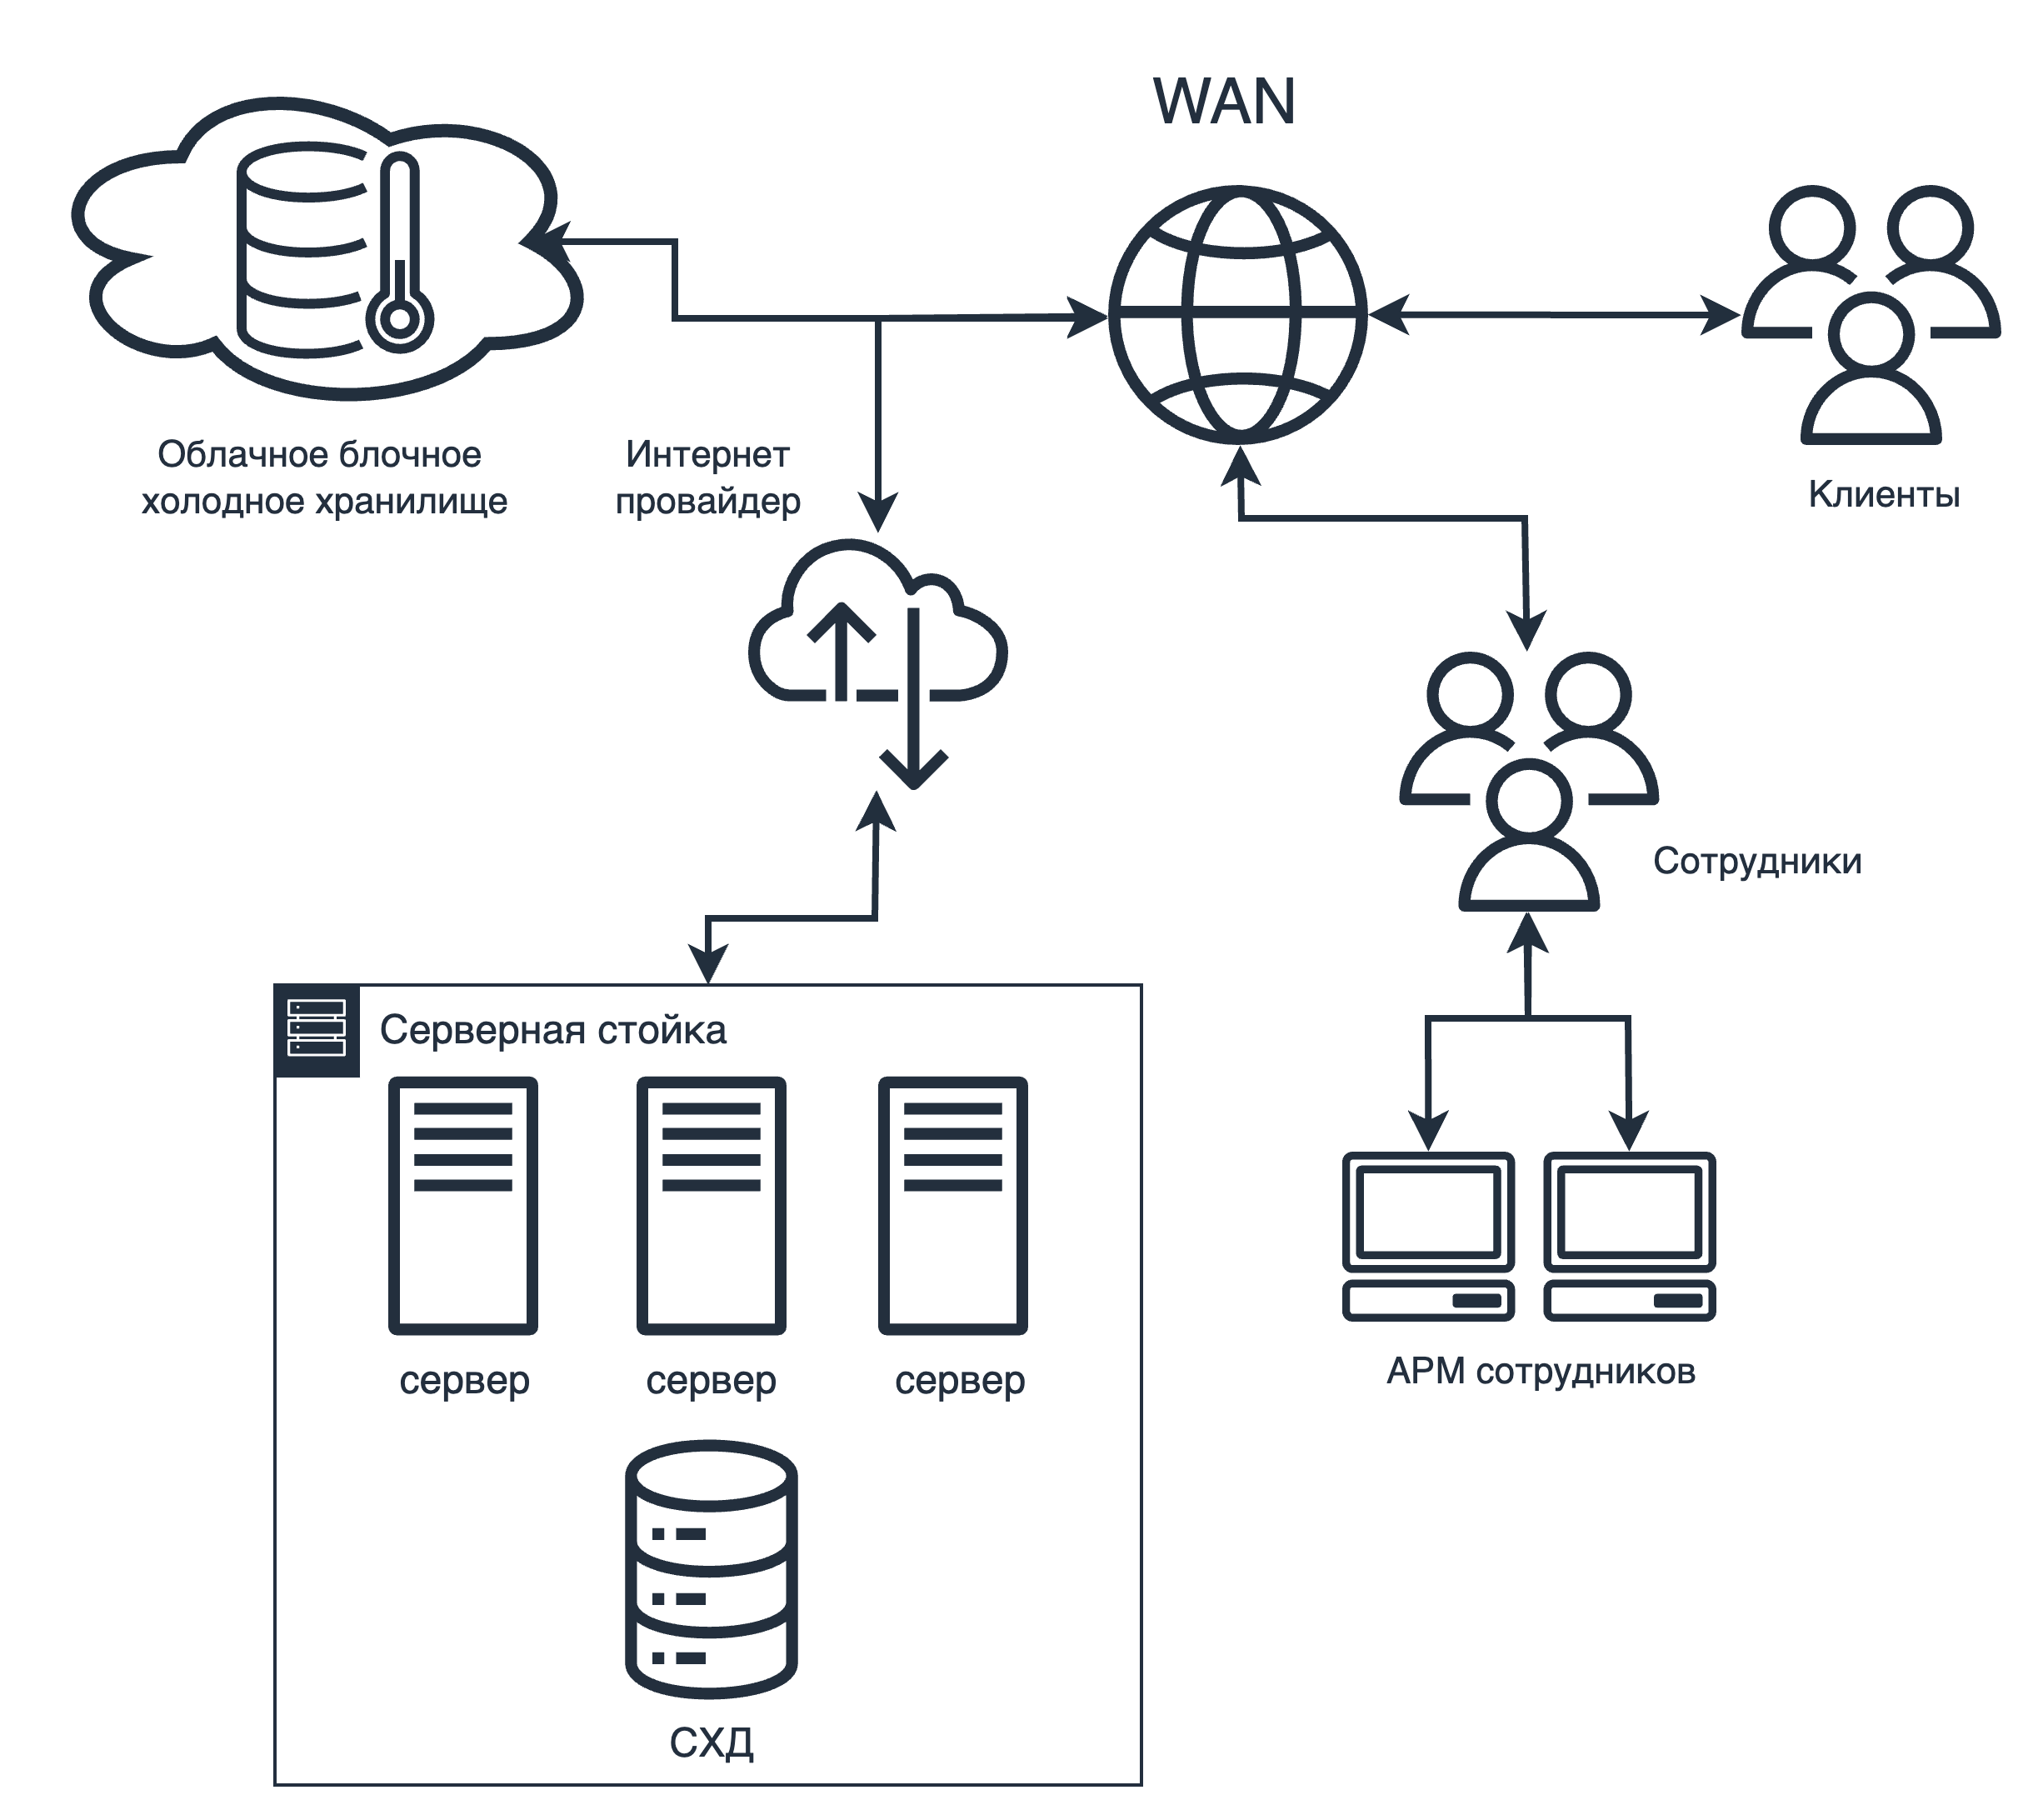
\includegraphics[width=0.9\textwidth]{infra2_2.png}
  \caption{Топология развертывания ИТ-инфраструктуры}
  \label{fig:infra2}
\end{figure}

\subsection{Системное и прикладное программное обеспечение}

Системное программное обеспечение (СПО) является важной частью проектируемой инфраструктуры,
так как системное ПО обеспечивает работоспособность ядра системы и взаимодействие между
аппаратными компонентами и прикладным ПО. В рамках проектируемой инфраструктуры
системы хранения и обработки данных ключевым СПО являются операционные системы
виртуальных машин и пользовательских устройств, гипервизоры, операционная система СХД
и так же могут входить в состав системного ПО системы резервного копирования и восстановления.

Прикладное программное обеспечение (ППО) является наиболее близким к конечному пользователью
и обеспечивает выполнение конкретных задач, таких как обработка данных, работа с
документами, взаимодействие с пользователем и т.д. В рамках проектируемой инфраструктуры
прикладным ПО является CRM-кредитования, скоринговая система и система сопровождения кредитов.

В качестве системы виртуализации и гипервизора выбрана система РЕД Виртуализация \cite{red-virtualization},
которая присутствует в реестре отечественного ПО, поддерживает резервное
копирование виртуальных машин, совместим с РЕД ОС, применяет алгоритмы шифромания
описанные в ГОСТ РФ и является полностью отечественной разработкой, которая
вполне может быть заменой программному обеспечению VMware vSphere\;\cite{wmware}.
Системные требования к оборудованию для РЕД Виртуализация приведены в
Таблице\;\ref{tab:hardware-requirements-red-virt} \cite{red-virtualization-system-requirements}.

\begin{tabularx}{\textwidth}{|l|X|X|}
  \caption{Минимальные и рекомендуемые требования к оборудованию для РЕД Виртуализация\label{tab:hardware-requirements-red-virt}}                \\
  \hline
  Конфигурация       & Минимальная                                            & Рекомендуемая                                                    \\\hline
  \endfirsthead
  \caption*{Продолжение таблицы~\ref{tab:hardware-requirements-red-virt}}                                                                        \\
  \hline
  Конфигурация       & Минимальная                                            & Рекомендуемая                                                    \\\hline
  \endhead
  \endfoot
  \endlastfoot

  Процессор          & Двухядерный процессор                                  & Четырехъядерный процессор или несколько двухъядерных процессоров \\\hline
  Оперативная память & 16 ГБ установленной оперативной памяти                 & 32 ГБ установленной оперативной памяти                           \\\hline
  Жесткий диск       & 80 ГБ доступного дискового пространства                & 100 ГБ доступного дискового пространства                         \\
  Сетевой интерфейс  & 1 сетевой интерфейс с пропускной способностью 1 Гбит/с & 1 сетевой интерфейс с пропускной способностью 10 Гбит/с          \\\hline
\end{tabularx}


В качестве операционной системы для виртуальных машин и для АРМ сотрудников выбрана
РЕД ОС \cite{red-os}, которая так же присутствует в реестре отечественного ПО.
Эта операционная система имеет две конфигурации <<Рабочая станция>> и <<Сервер>>.
Конфигурация <<Рабочая станция>> имеет интуитивно понятный интерфейс, встроенные
офисные приложения, бразуеры и приложения для работы с документами, что отлично
подходит для АРМ сотрудников. Преимуществами конфигурации <<Сервер>> является
возможность построения домена на базе Samba DC, кластеры высокой доступности
и программно определяемые системы хранения данных, что для будущего развития
и масштабирования инфраструктуры может являться важной деталью. Системные требования
для РЕД ОС в конфигурациях <<Сервер>> и <<Рабочая станция>> приведены в
Таблице\;\ref{tab:redos-system-requirements} \cite{red-os-system-requirements}.

\begin{tabularx}{\textwidth}{|l|X|X|X|}
  \caption{Системные требования для РЕД ОС 7.3 и 8\label{tab:redos-system-requirements}}                                          \\
  \hline
  Конфигурация                    & Рабочая станция               & Сервер                        & Сервер минимальный            \\\hline
  \endfirsthead
  \caption*{Продолжение таблицы~\ref{tab:redos-system-requirements}}                                                              \\
  \hline
  Конфигурация                    & Рабочая станция               & Сервер                        & Сервер минимальный            \\\hline
  \endhead
  \endfoot
  \endlastfoot

  Процессор                       & x86\_64 1{,}6 ГГц 2 ядра      & x86\_64 1{,}6 ГГц 2 ядра      & x86\_64 1{,}6 ГГц 1 ядро      \\\hline
  Оперативная память              & 2 ГБ                          & 2 ГБ                          & 1 ГБ                          \\\hline
  Свободное дисковое пространство & 20 ГБ                         & 20 ГБ                         & 8 ГБ                          \\\hline
  Видеоадаптер                    & Поддержка режима SVGA 800×600 & Поддержка режима SVGA 800×600 & Поддержка режима SVGA 800×600 \\\hline
\end{tabularx}


Системное ПО используемое для СХД -- это программное обеспечение RAIDIX серии 5.2.
RAIDIX это Россйская разработка, которая явялется одним из лидеров в области систем хранения
данных. Оснобенностью RAIDIX является то, что он позволяет создавать гибридные и
all-flash СХД с высокоскоростным блочным (SAN) и файловым (NAS) доступом, кроме того
в СХД он позволяет работать с такими уровнями RAID, как 0, 1, 5, 6, 7.3, 10, 50, 60, 70, N+M.

Выбор в сторону отечественного системного ПО обусловлен тем, что это в первую очередь дешевле,
кроме того это полностью соответствует требованиям испортозамещения. На Россйском
рынке имеется большое количество специалистов, которые могут поддерживать это ПО
в отличии от зарубежных аналогов, которые требуют высококвалифицированных специалистов
которым так же требуется высокая оплата труда.

В предоженной инфраструктуре в роли прикладного ПО используется CRM система <<Битрикс24>>
\cite{bitrix24} для управления бизнес-процессом кредитования c дополнительными модулями
<<бизнес-процессы>> для автоматизации этапов запуска скоринга и автоматические напоминания
сотрудникам, <<Документооборот>> для генерации документов, <<Аналитика и отчеты>>
для проведения анализа и составления отчетов по ним. Стоит учитывать, что количество
дополнительных модулей может изменяться в зависимости от потребностей бизнеса, а
это значит, что расчет по системным требованиям может изменяться и стоит предусмотреть возможный
рост нагрузки на систему. Исходя из данных о количестве активных пользователей составляющей
800 человек и количестве записей от 3000-5000 в день. Данные о количестве пользователей
и операций в день позволяют сформировать системные требования, которые рассчитаны с учетом
на будущее масштабирование и приведены в Таблице\;\ref{tab:bitrix-system-requirements} \cite{bitrix24-system-requirements}.


\begin{tabularx}{\textwidth}{|l|X|X|}
  \caption{Системные требования для установки Битрикс24 с модулями CRM \label{tab:bitrix-system-requirements}}         \\
  \hline
  Конфигурация                    & Минимальные требования                 & Рекомендуемые требования                  \\\hline
  \endfirsthead
  \caption*{Продолжение таблицы~\ref{tab:bitrix-system-requirements}}                                                  \\
  \hline
  Конфигурация                    & Минимальные требования                 & Рекомендуемые требования                  \\\hline
  \endhead
  \endfoot
  \endlastfoot

  Процессор                       & 6 ядра, 2{,}0 ГГц                      & 8 ядер, 2{,}4 ГГц и выше                  \\\hline
  Оперативная память              & 32 ГБ                                  & 64 ГБ                                     \\\hline
  Свободное дисковое пространство & 500 ГБ SSD                             & 1 ТБ NVMe SSD                             \\\hline
  Операционная система            & Linux (CentOS 7/8, Ubuntu 20.04/22.04) & Linux (Ubuntu LTS, RHEL)                  \\\hline
  СУБД                            & MySQL 5.7 / MariaDB 10.5               & MariaDB 10.6--10.11, кластеризация        \\\hline
  Сетевое подключение             & Порт 1 Gbps                            & Выделенный канал 1 Gbps с резервированием \\\hline
\end{tabularx}


Скоринговая система является еще одним прикладным программным обеспечением в проектируемой
инфраструктуре, так как она отвечает за автоматизацию процесса оценки кредитоспособности
клиентов и принятия решений о выдаче кредита. Скоринговая система позволяет
сократить время обработки заявок, повысить точность оценки рисков и снизить
количество ошибок. Все вышеперечисленные факторы и характеристики говорят о том,
что скоринговая система представляет из себя большой комлекс программных решений,
которые крайне требовательны к ресурсам и требуют высокой производительности,
кроме того масштабируемость важна для этого ПО, так как объем данных стремительно
растет и требует все больше ресурсов для хранения и обработки. Системные требования
для ПО скоринговой системы приведены в Таблице\;\ref{tab:scoring-system-requirements}.
Стоит обратить внимание на то, что объем памяти указан для самого ПО, а
пользовательские данные занимают 5ТБ.

\begin{tabularx}{\textwidth}{|l|X|X|}
  \caption{Системные требования для ПО кредитной скоринговой системы \label{tab:scoring-system-requirements}} \\
  \hline
  Конфигурация                    & Рекомендуемые требования                                                  \\\hline
  \endfirsthead
  \caption*{Продолжение таблицы~\ref{tab:scoring-system-requirements}}                                        \\
  \hline
  Конфигурация                    & Рекомендуемые требования                                                  \\\hline
  \endhead
  \endfoot
  \endlastfoot

  Процессор                       & 18 ядер, 2{,}5 ГГц и выше                                                 \\\hline
  Оперативная память              & 56 ГБ                                                                     \\\hline
  Свободное дисковое пространство & 3 ГБ NVMe SSD                                                             \\\hline
  Операционная система            & Linux                                                                     \\\hline
  СУБД                            & PSQL, MongoDB, кластеризация                                              \\\hline
\end{tabularx}

Система поддержки кредитов является еще одним прикладным программным обеспечением
в проектируемой инфраструктуре, так как она отвечает за автоматизацию процесса
сопровождения кредитов, включая управление платежами, отслеживание задолженности
и взаимодействие с клиентами. Это означает, что система должна на постоянной основе
с большой частотой скнировать базы данных и обрабатывать большие объемы данных,
которые постоянно растут. Требования к системе поддержки кредитов представлены
в Таблице\;\ref{tab:credit-support-system-requirements}. Система поддержки кредитов
обрабатывает те же самые пользовательские данные, что и скоринговая система.

\begin{tabularx}{\textwidth}{|l|X|X|}
  \caption{Системные требования для ПО поддержки кредитов\label{tab:credit-support-system-requirements}} \\
  \hline
  Конфигурация                    & Рекомендуемые требования                                             \\\hline
  \endfirsthead
  \caption*{Продолжение таблицы~\ref{tab:credit-support-system-requirements}}                            \\
  \hline
  Конфигурация                    & Рекомендуемые требования                                             \\\hline
  \endhead
  \endfoot
  \endlastfoot

  Процессор                       & 16 ядер, 2{,}4 ГГц и выше                                            \\\hline
  Оперативная память              & 56 ГБ                                                                \\\hline
  Свободное дисковое пространство & 3  ГБ NVMe SSD                                                       \\\hline
  Операционная система            & Linux                                                                \\\hline
\end{tabularx}

Топология развертывания ЦОД с указанием СПО приведена на Рисунке\;\ref{fig:deployment_server}.

\begin{figure}[H]
  \centering
  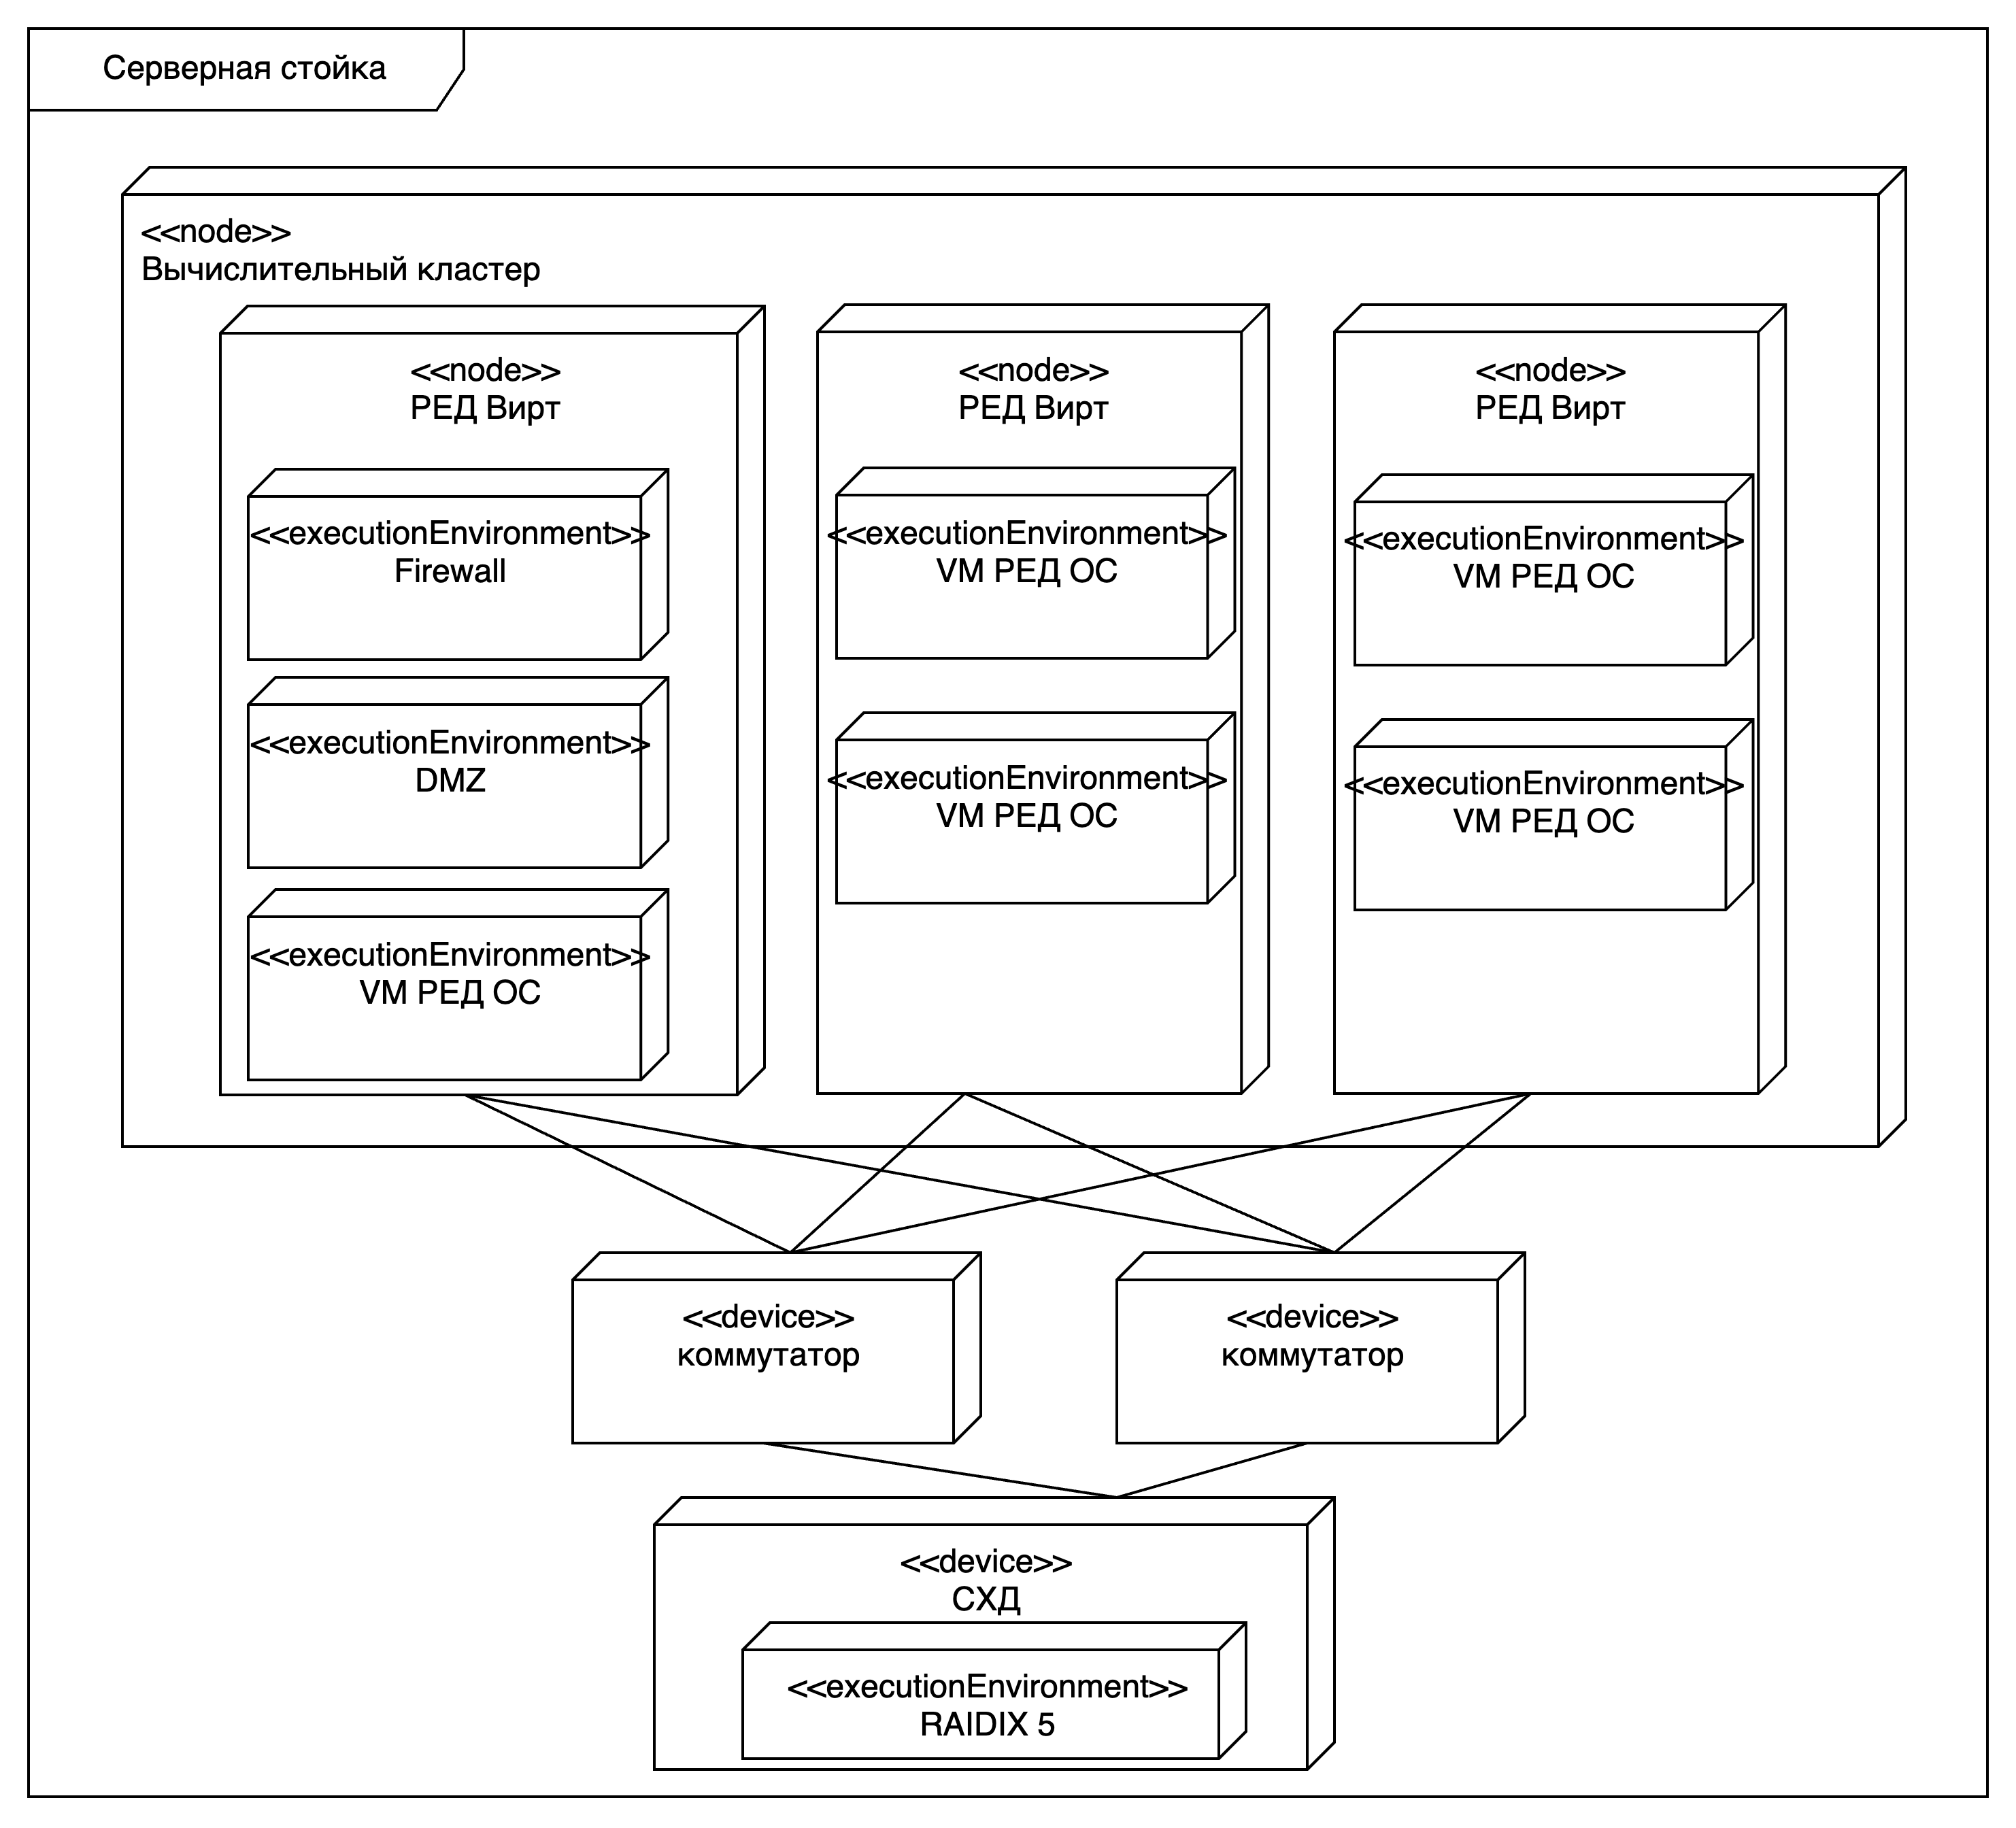
\includegraphics[width=0.9\textwidth]{deployment_server.png}
  \caption{Топология развертывания ЦОД с указанием СПО}
  \label{fig:deployment_server}
\end{figure}

Топология развертывания АРМ сотрудников с указанием СПО приведена на Рисунке\;\ref{fig:deployment_arm}.

\begin{figure}[H]
  \centering
  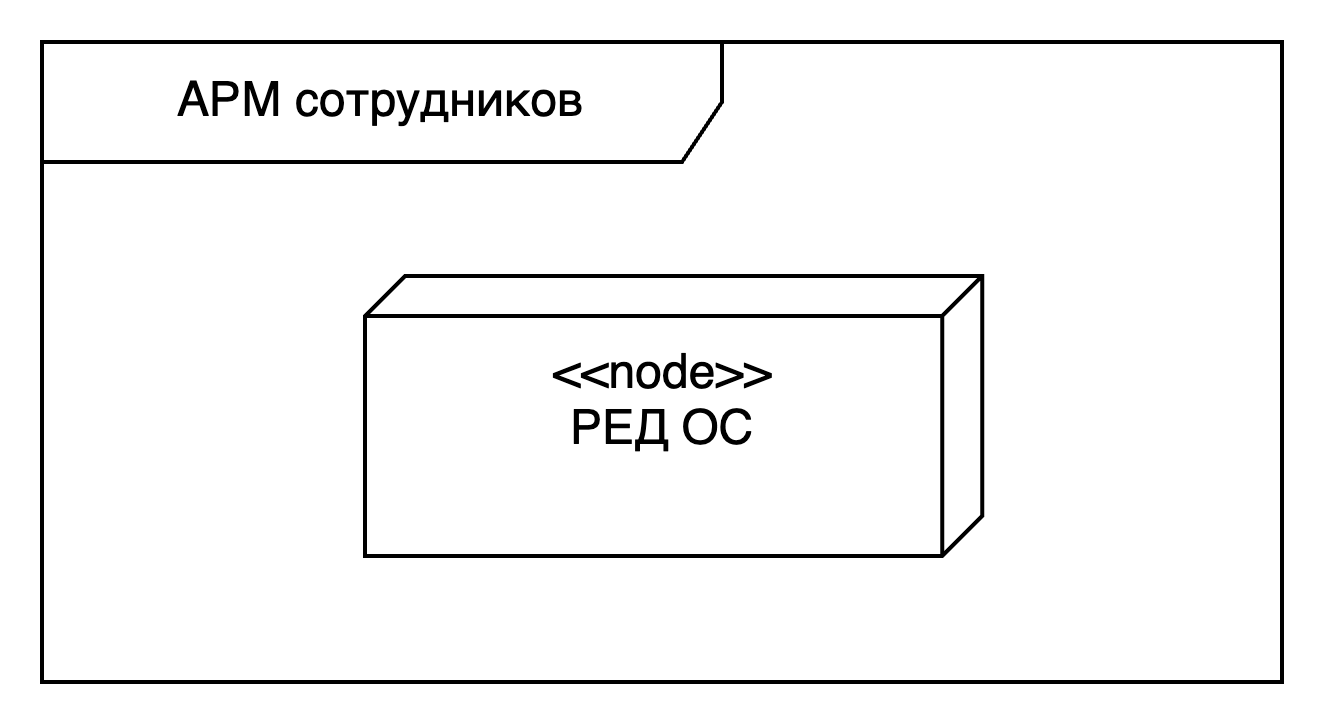
\includegraphics[width=0.5\textwidth]{deployment_arm.png}
  \caption{Топология развертывания АРМ сотрудников с указанием СПО}
  \label{fig:deployment_arm}
\end{figure}


В Таблице \;\ref{tab:summary-system-requirements} представлены системные требования всех компонентов
инфраструктуры без учета пользовательских данных для хранлищ и реплик баз данных.


\begin{tabularx}{\textwidth}{|l|X|X|X|X|X|X|}
  \caption{Общие системные требования\label{tab:summary-system-requirements}}                                                                    \\
  \hline
  №  & Название ПО        & Тип ПО             & Назнчание ПО           & Требование к CPU, ядер & Требования к ОЗУ, ГБ & Требования к диску, ГБ \\ \hline
  \endfirsthead
  \caption*{Продолжение таблицы~\ref{tab:summary-system-requirements}}                                                                           \\
  \hline
  №  & Название ПО        & Тип ПО             & Назнчание ПО           & Требование к CPU, ядер & Требования к ОЗУ, ГБ & Требования к диску, ГБ \\ \hline
  \endhead
  \endfoot
  \endlastfoot

  1  & Битрикс24          & Прикладное         & CRM система            & 8                      & 64                   & 1000                   \\ \hline
  2  & Скоринговая        & Прикладное         & Банковская система     & 18                     & 56                   & 3                      \\ \hline
  3  & Поддержка кредитов & Прикладное         & Банковская система     & 16                     & 56                   & 3                      \\ \hline
  4  & РЕД Вирт           & Системное          & Гипервизор             & 4                      & 32                   & 100                    \\ \hline
  5  & РЕД ОС             & Системное          & ОС                     & 2                      & 2                    & 20                     \\ \hline
  6  & Zabbix             & Инструме- нтальное & Мониторинг             & 4                      & 16                   & 100                    \\ \hline
  7  & Grafana            & Инструме- нтальное & Мониторинг             & 4                      & 8                    & 50                     \\ \hline
  8  & Prometheus         & Инструме- нтальное & Метрики                & 4                      & 8                    & 100                    \\ \hline
  9  & PostgreSQL         & Инструме- нтальное & База данных            & 8                      & 32                   & 10                     \\ \hline
  10 & РЕД АДМ            & Инструме- нтальное & Управление и настройка & 4                      & 4                    & 100                    \\ \hline
  11 & RuBackup           & Инструме- нтальное & СРК                    & 4                      & 4                    & 480                    \\ \hline
  12 & Kubernetes Cluster & Инструме- нтальное & Контей- неризация      & 8                      & 64                   & 150                    \\ \hline
\end{tabularx}


\subsection{Инструментальное программное обеспечение}

Инструментальное программное обеспечение - это совокупность программ, предназначенных для
разработки, тестирования, сопровождения и эксплуатации других программных средств и
информационных систем. Инструментальное программное обеспечние в инфраструктуре заключается
в таких системах, как сбор метрик, конфигурационное управление, контейнеризация,
СУБД, система бэкпирования и не только.

Основная СУБД используемая банковскими сервисами предоставляемыми как прикладное ПО
является PostgreSQL. Это объектно-реляционная система управления базами данных (ORDBMS),
наиболее развитая из СУБД с открытым исходным кодом в мире и является альтернативой
коммерческим базам данных. Именно это СУБД используется для обработки всех клиентских
данных объем которых явялется наиболее большим в инфраструктуре. Так как на нее приходится
большая нагрузка из-за объема данных, то она будет развернута в том числе в виде репили, а
это означает, что под реплику выделена еще одна отдельная виртуальная машина.

Системы сбора и отображения метрик состоят из трех програминых комплексов, такиз как Zabbix,
Grafana и Prometheus. Основным из них является zabbix, так как именно он применяется для
отслеживания состояния и производительности сетевых интерфейсов, серверов и виртуальных машин.
Grafana и Prometheus же применяются для сбора метрик состояния и производительности приложений.
Zabbix \cite{zabbix} и все остальные сервисы мониторинга развернуты на одной виртуальной машине внутри кластера РЕД.
Собираемые метрики по СХД включают в себя свободное и заятое пространство, производительность,
состояние дисков и температуру контроллеров. Метрики по критичным данным, таким как паять и доступность
и производительность дисков собираются каждые 2 минуты, занятость памяти и состояние пулов СХД
каждые 6 минут, а роcт данных и износ дисков каждые 2 часа.

Как система централизованного управления ИТ-инфраструктурой используется программный комплекс
РЕД АДМ. Он позволяет администрировать инфраструктуру со смешанным набором ОС используя
ansible через веб-интерфейс с широким набором инструментов и является масштабируемым и
отказаустойчивым ПО при росте нагрузке, что явялется критическим для инфраструктуры информационного
сервиса банка.

Для автоматизации и аркестрации управления контейнеризированными приложениями модуля кредитования
информационной системы используется Kubernetes \cite{k8s}. Контейнеры для развертывания кластера Kubernetes
размещены на разных физических узлах внутри кластера РЕД вирт, что обеспечивает распределение нагрузки
и дополнительную отказаустойчивость в случае отказа какого-либо из компонентов инфраструктуры.

В роли системы резервного копирования используется отвечественное программное средство RuBackup.
RuBackup это ПО назначенное для создания резервных копий данных, виртуальных машин, баз данных
рабочих станций и серверов с возможностью их быстрого восстановления. ПО полностью соответствует
Россйиским требованиям безопасности и (152-ФЗ). Он собирает все данные хранящиеся на локальном СХД
и дублирует их на облачное блочное хранилище.

\subsection{Сетевая инфраструктура}

Разработка сетевой инфраструктуры для модуля поддержки потребительского кредитования информационной
системы кредитной организации направлена на обеспечение надежной, безопасной и масштабируемой
передачи данных между компонентами ИТ-инфраструктуры. Сетевая инфраструктура выступает основой
для интеграции локального центра обработки данных (ЦОД) и облачных ресурсов, обеспечивая выполнение
требований по доступности, производительности и безопасности, определенных в рамках целевых уровней
качества обслуживания (SLA). В данном разделе рассматриваются состав сетевых служб, сетевая топология,
спецификации сетевого оборудования, схемы адресации узлов и распределения доменных имен, а также
конфигурации сетевых сервисов.

Так как ЦОД заключается в аренде серверной стойки с применеием модели colocation у
вендора, то такие сетевые устройства как маршрутизатор и коммутаторы расположены в той же
серверной стойке что и сами серверы и СХД.

В состав стевых служб входят DHCP, NTP, DNS, межсетевой экран.

NTP и DNS предоставляются системой РЕД АДМ, там же происходит удобная конфигурация
с исопльзованием пользовательского интерфейса.

Выбранный маршрутизатор -- это ESR-3300 от производителя Eltex, который представляет собой
универсальную аппаратную платформу и способное выполнять широкий круг задач,
связанных с сетевой защитой, шифрованием передаваемых данных,
терминированием пользователей и т. д. Маршрутизатор состоит из 4 портов 1000BASE-X/10GBASE-R/25GBASE-R (LAN/WAN) и
4 портов 40GBASE-R QSFP+/100GBASE-R QSFP28. DHCP так же насроен на маршрутизаторе.

Коммутаторы L3 и L2 выбраны так же от производитя Eltex, а именно модель MES5324. Данная модель
коммутатора имеет 24 порта 10Гбит/с (SFP+) и 4 порта 40Гбит/с этого достаточно, чтобы на
данный момент обеспечить подключение всех компонентов инфраструктуры и заложить
под будущее масштабирование. Количество таких коммутаторов 3, так как один из них
используется на уровне ядра и еще 2 на уровне агрегации.

Посколько соединение СХД с севером осуществлется с использованием фабрики, она стоит из двух
SAN коммутаторов к каждой из которых имеется соединение от обоих контроллеров СХД, а коммутаторы
в свою очередь соеденены с каждым из серверов. Наиболее подходящий вариант коммутатора предоставляется
вендором Dell модель DS-6610B. Это SAN коммутатор поддерживащий пропускную способность до 760 Гбит/с
и 24 порта скоростью 32Gb SFP+.

Топология сети c устройствами и их схемой адресов представленной на Рисунке\;\ref{tab:marshrut}
представлена на Рисунке\;\ref{fig:togo-network}.

\begin{tabularx}{\textwidth}{|X|X|X|X|}
  \caption{Схема адресации устройств внутри ЦОД\label{tab:marshrut}} \\
  \hline
  Устройство         & IP адрес      & Доменное имя     & ID VLAN    \\ \hline
  \endfirsthead
  \caption*{Продолжение таблицы~\ref{tab:marshrut}}                  \\
  \hline
  Устройство         & IP адрес      & Доменное имя     & ID VLAN    \\ \hline
  \endhead
  \endfoot
  \endlastfoot

  Server\_1          & 126.126.1.2   & server1.dc.local & 20         \\ \hline
  Server\_2          & 126.126.1.3   & server2.dc.local & 20         \\ \hline
  Server\_3          & 126.126.1.4   & server3.dc.local & 20         \\ \hline
  LAN\_Switch\_L2\_1 & 126.126.2.2   & sw1.l2.dc.local  & 30         \\ \hline
  LAN\_Switch\_L2\_2 & 126.126.2.3   & sw2.l2.dc.local  & 30         \\ \hline
  LAN\_Switch\_L3\_1 & 126.126.3.2   & sw1.l3.dc.local  & 40         \\ \hline
  LAN\_R\_1          & 126.126.4.2   & r1.dc.local      & 50         \\ \hline
  SAN\_Switch\_1     & 126.126.242.2 & sw1.fb.dc.local  & -          \\ \hline
  SAN\_Switch\_2     & 126.126.242.3 & sw2.fb.dc.local  & -          \\ \hline
\end{tabularx}

\begin{figure}[H]
  \centering
  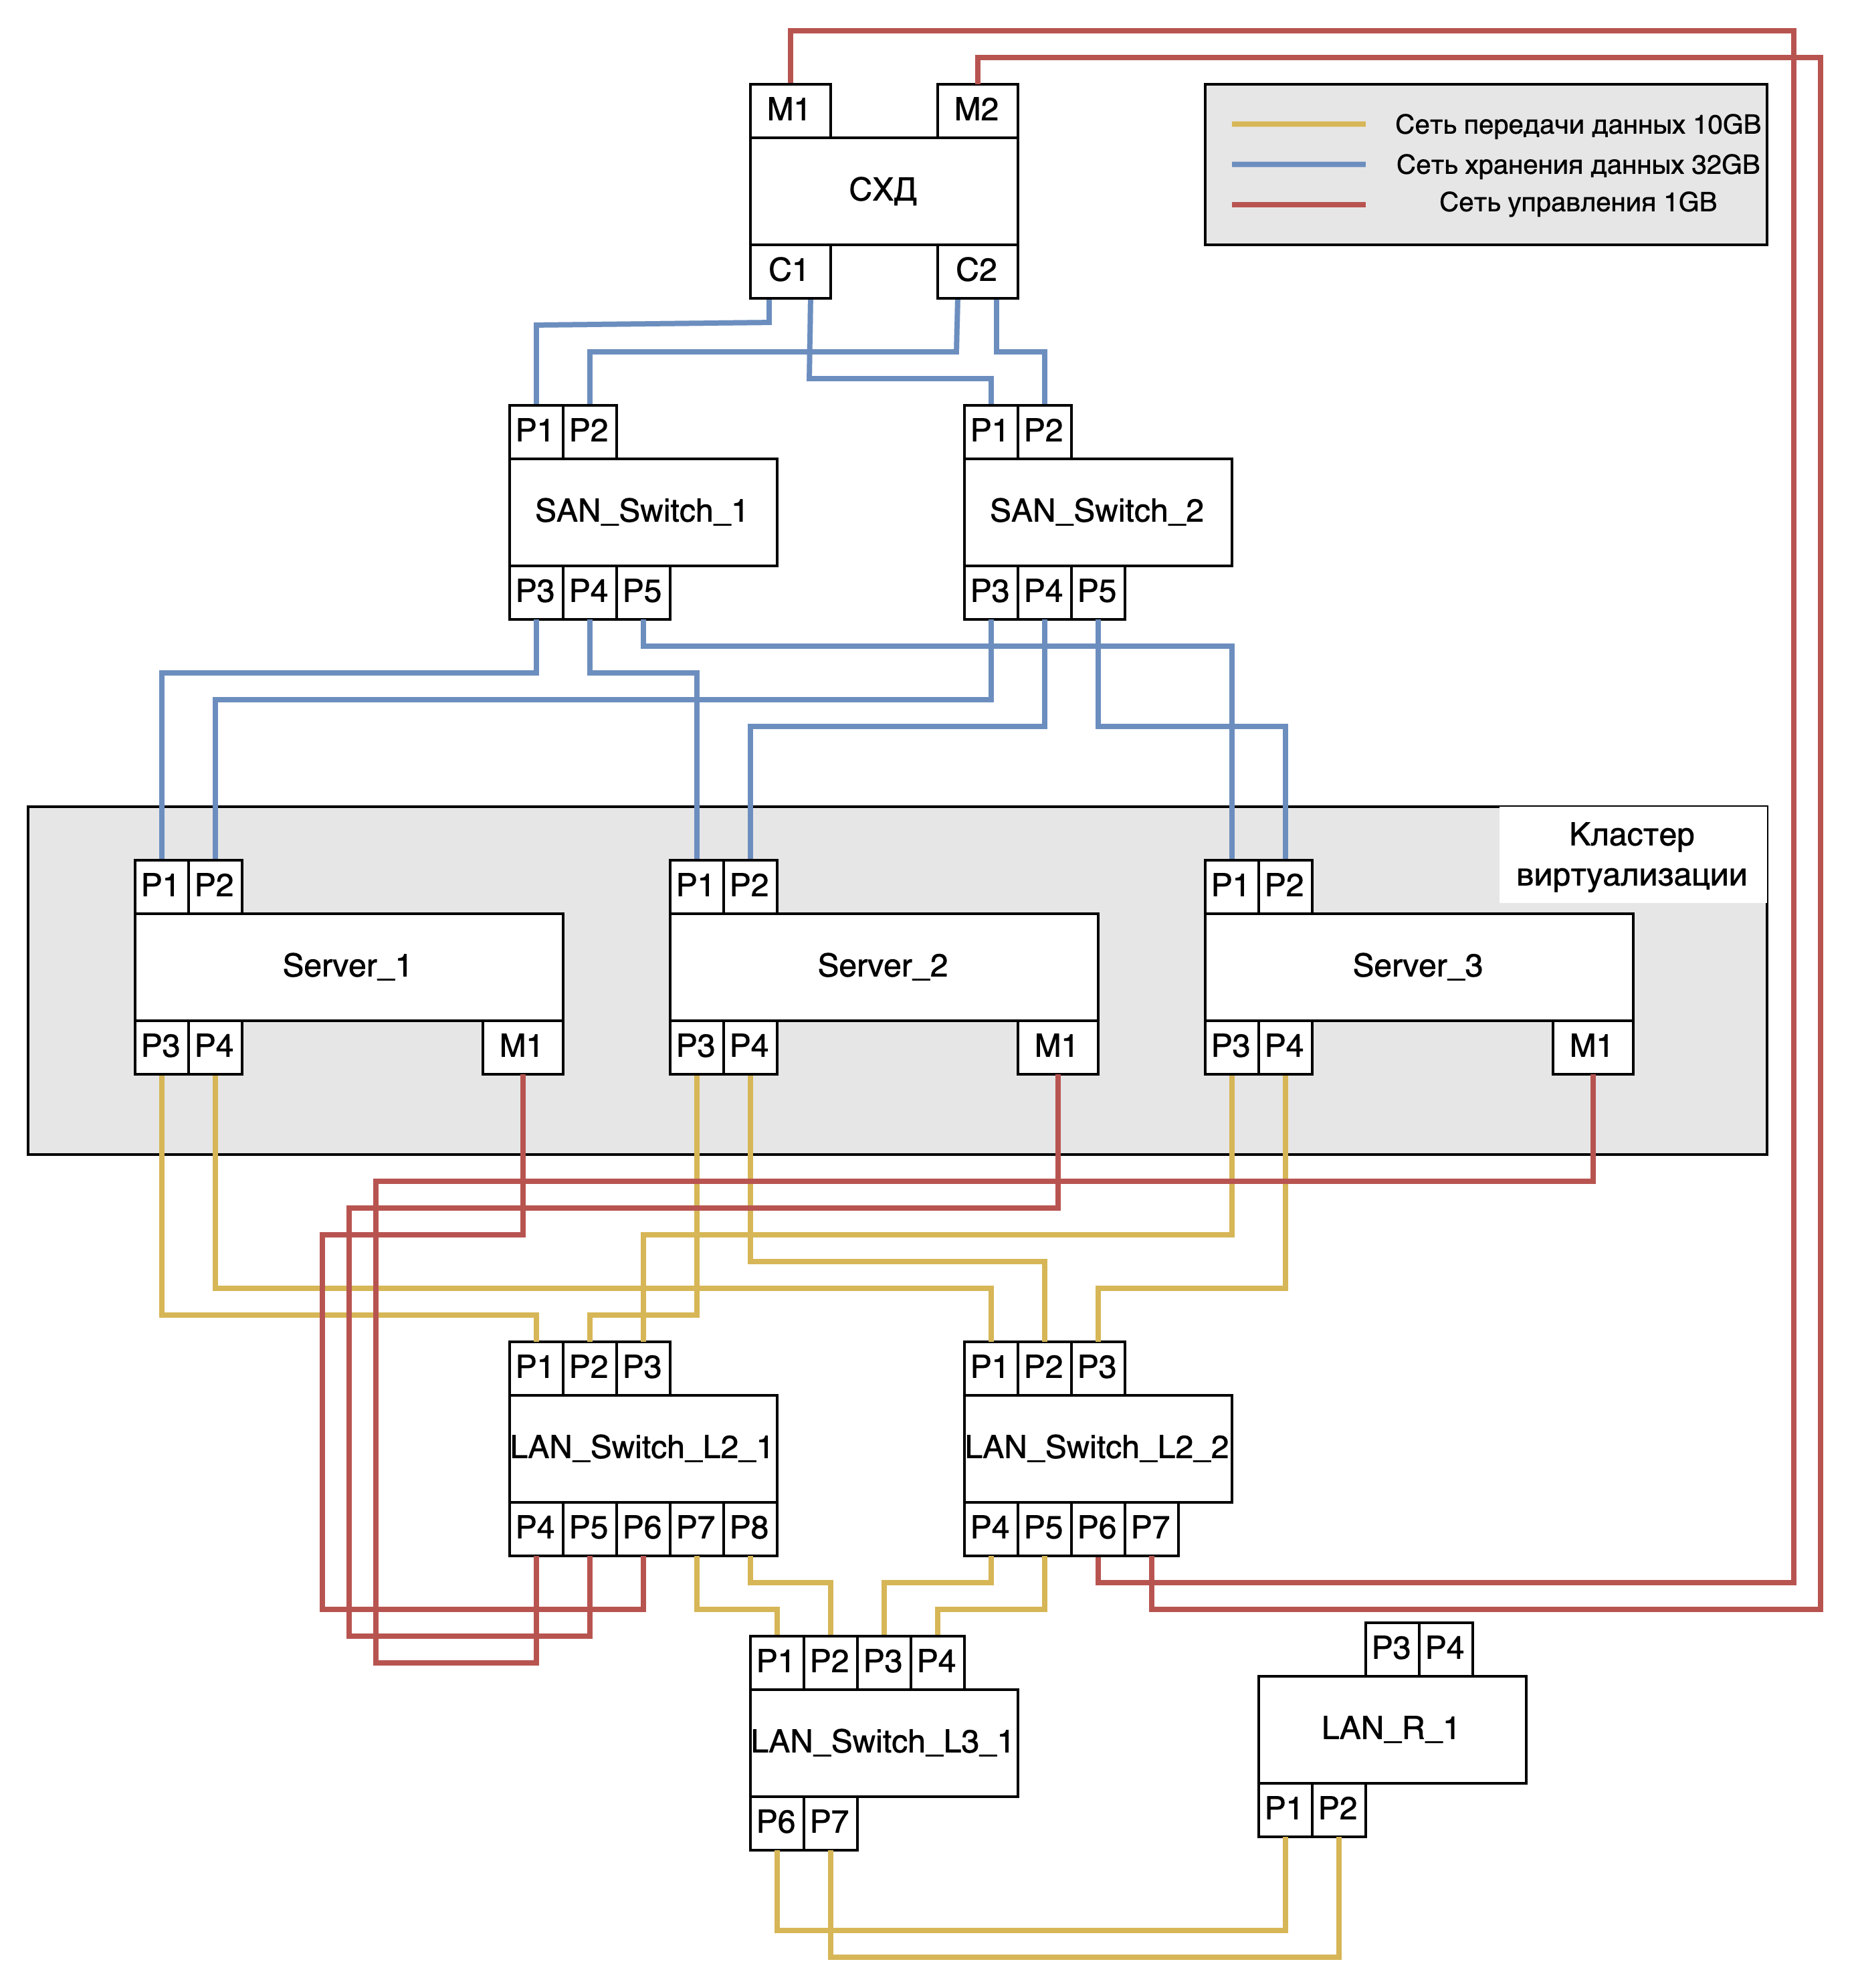
\includegraphics[width=0.9\textwidth]{net_topo.png}
  \caption{Топология сети ЦОД}
  \label{fig:togo-network}
\end{figure}

\subsection{Техническое обеспечение}

Техническое обеспечение включает серверное оборудование, системы хранения данных, клиентские устройства,
периферийное оборудование, а также системы электроснабжения, кондиционирования и пожаротушения. В условиях
использования модели colocation, предполагающей аренду серверной стойки у вендора, акцент сделан на
оптимизации размещения оборудования, минимизации энергопотребления и обеспечении соответствия нормативным
требованиям. В данном разделе приводятся спецификации серверов, рабочих мест пользователей и систем
хранения данных, схема размещения оборудования в стойках, расчет энергопотребления с учетом источников
бесперебойного и резервного питания, а также требования к системам кондиционирования и пожаротушения.
Проектирование осуществляется с учетом необходимости обеспечения высокой доступности, безопасности
данных и возможности масштабирования инфраструктуры.

Все техническое обеспение предложеноое в пункте о компонентах инфраструктуры по итогам расчетов
технических требований системного, прикладного и специального ПО верны, так как они рассчитны на
обработку именно такого объема данных с дальнейшим масшиабированием. К используемым периферйным устройствам
можно отнести HBA-адаптер для каждого из серверов, который используется для формирования фабрики
между самим сервером и СХД.

Так как серверная инфраструктура полностью расположена в одной серверной стойке арендуемой у вендора
Selecte, то системы электроснабжения, кондиционирования и пожаротушения так же предоставляются им.
Базовый пакет услуг collocation включает в себя 5КВА мощности с условием, что дополнительные мощности
можно приобрести с оплатой, так же в базоывй пакет входят 2 независимых луча электропитания, что
обеспечивает бесперебойное энергоснабжение. Итоговая таблица тхенического
обеспечения с сетевыми устройствами их потреблением мощности представлена в Таблице\;\ref{tab:technical_infrastructure_power}

\begin{tabularx}{\textwidth}{|l|X|c|}
  \caption{Итоговая таблица технического обеспечения с потреблением электроэнергии\label{tab:technical_infrastructure_power}} \\
  \hline
  Оборудование                 & Потребление электроэнергии, Вт & Количество                                                  \\\hline
  \endfirsthead
  \caption*{Продолжение таблицы~\ref{tab:technical_infrastructure_power}}                                                     \\
  \hline
  Компонент                    & Потребление электроэнергии, Вт & Количество                                                  \\\hline
  \endhead
  \endfoot
  \endlastfoot

  Сервер «Гравитон» С2122ИУ    & 350                            & 3                                                           \\ \hline
  СХД «Гравитон» СХ424И24БМ-РЭ & 1200                           & 1                                                           \\ \hline
  Коммутатор Eltex MES5324     & 240                            & 3                                                           \\ \hline
  Dell DS-6610B                & 77                             & 2                                                           \\ \hline
  Маршрутизатор     ESR-3300   & 177                            & 1                                                           \\ \hline
  Итого                        & 3300                           & 10                                                          \\ \hline
\end{tabularx}

Итоговое энергопотребеление составляет 3300 Вт, что равняет 3,3 кВт. Это означает,
что предоставляемого количества вендором достаточно для поддержвания существущей
инфраструктуры в том числе с будущим масштабированием.

Серверная стойка с компоновкой всех физических компонентов инфраструктуры внутри стойки
приведены на Рисунке\;\ref{fig:server_rack}

\begin{figure}[H]
  \centering
  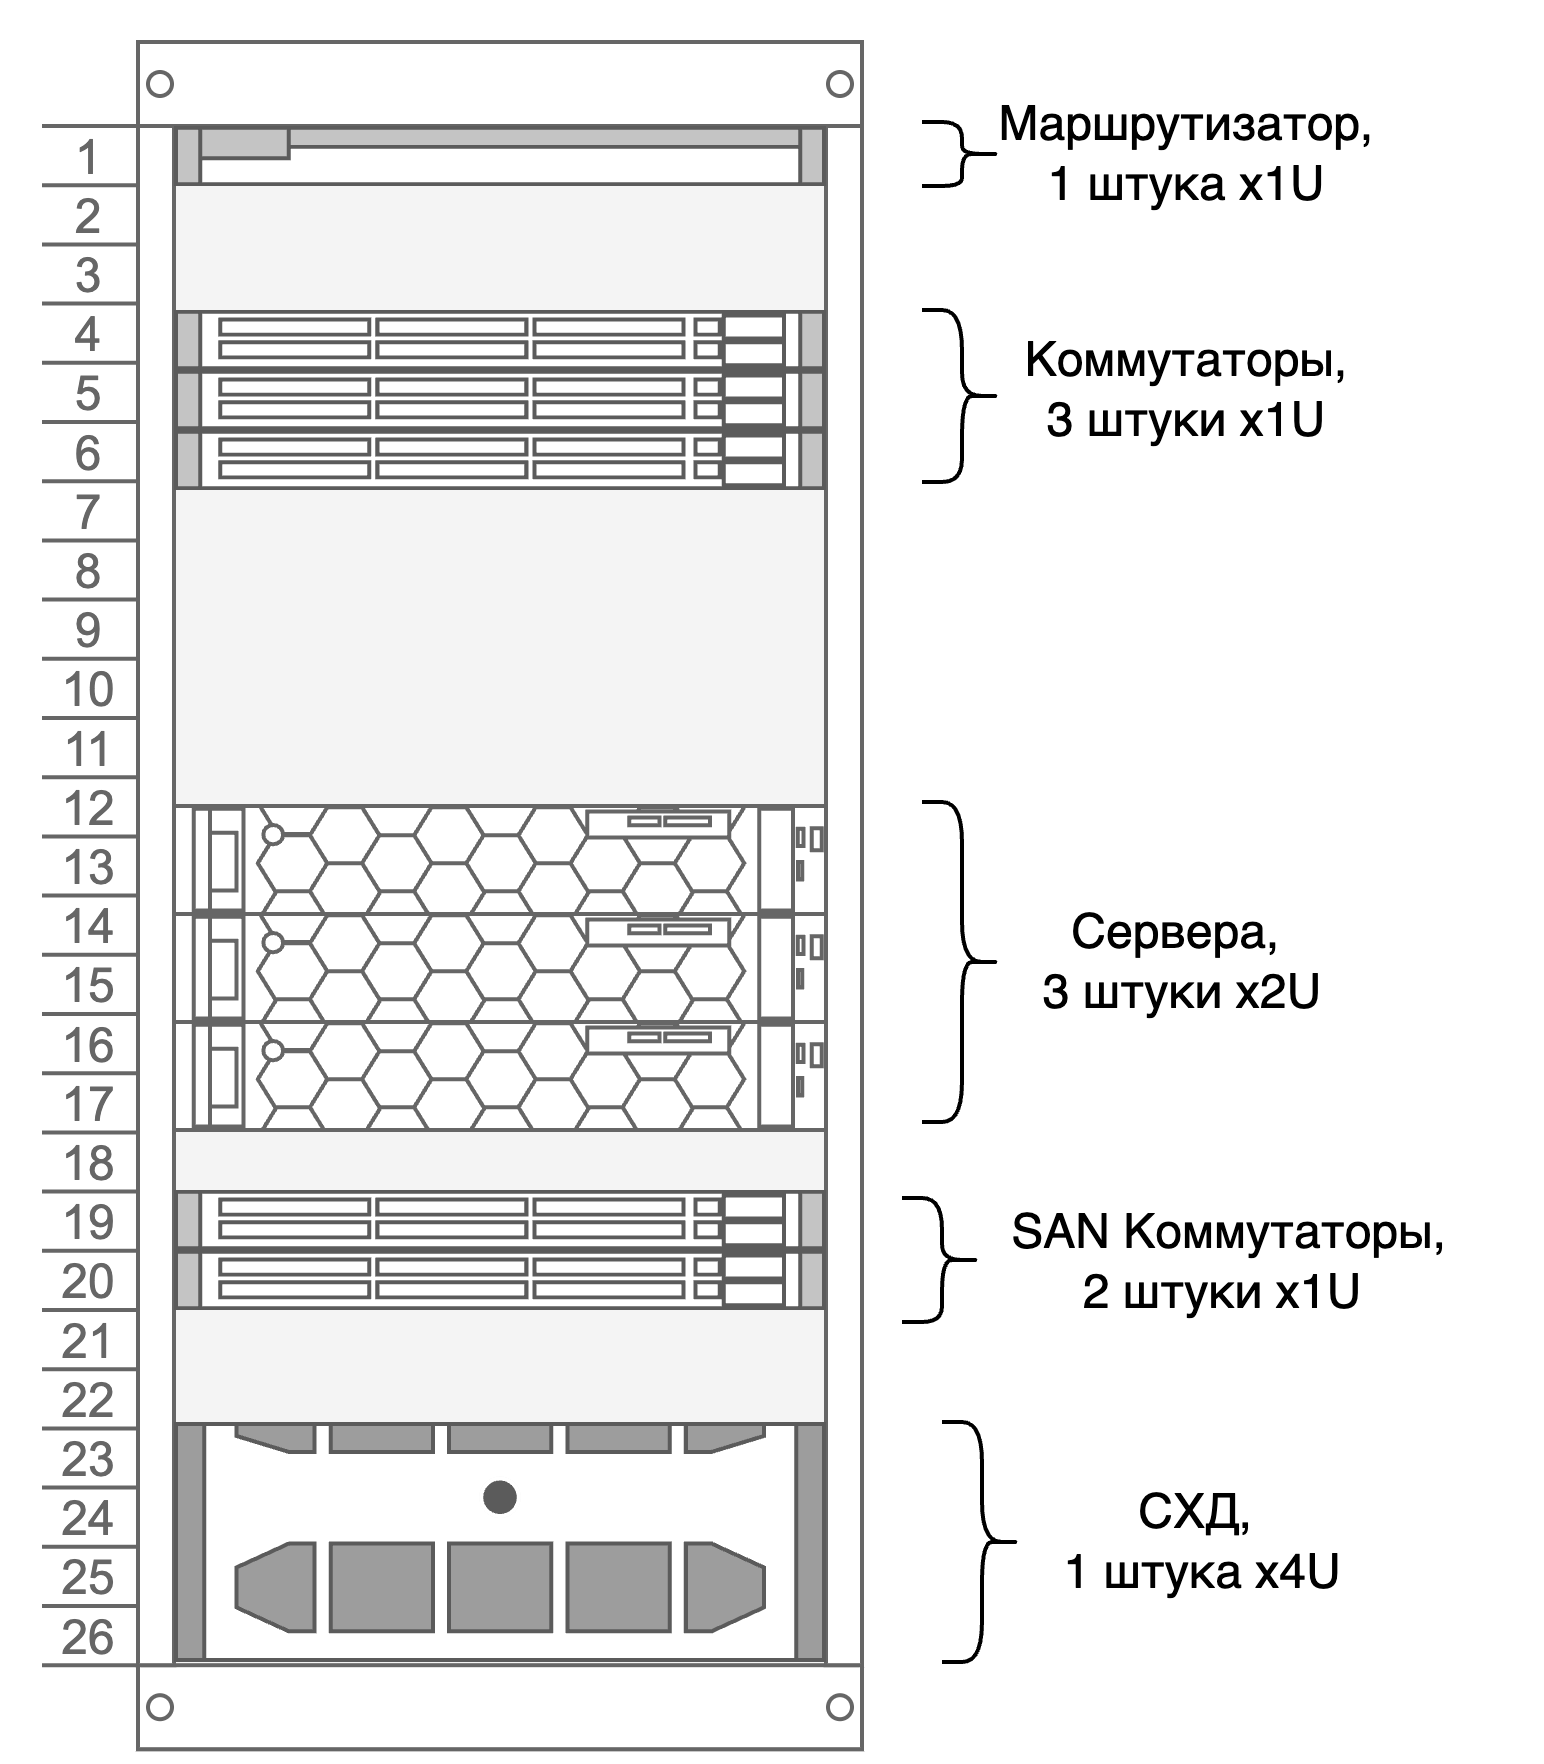
\includegraphics[width=0.9\textwidth]{server_rack.png}
  \caption{Серверная стойка}
  \label{fig:server_rack}
\end{figure}

Автоматизированные работчие места (АРМ) сотрудников - это корпоративные ноутбуки, которые
являются опциольными для сотрудников, так как все сотрудники компании работют удаленно.
В связи с этим, для проектируемой инфраструктуры выбраны ноутбуки <<Aquarius AQbook NE355>> \cite{aquarius-aqbook-NE355}.
Ноутбук поддерживает процессор AMD ryzen 5600, до 64 ГБ оперативной памяти и от 256 ГБ
постоянной памяти. Тот факт, что это ноутубки Российского производства позволяет
иметь быстрое сервисоное обслуживание и поддержку.

\subsection{Организационное обеспечение}

В условиях использования модели colocation с арендой серверной стойки в центре
обработки данных акцент сделан на создании оптимальной организационной модели,
учитывающей специфику локального развертывания. В данном разделе рассматривается
штатная структура отдела сопровождения ИТ-инфраструктуры, включающая роли,
обязанности и квалификационные требования персонала, необходимые для эксплуатации
и поддержки проектируемой инфраструктуры. Проектирование организационного обеспечения
осуществляется с учетом потребностей в обеспечении отказоустойчивости, безопасности
данных и оперативного реагирования на инциденты, а также минимизации эксплуатационных рисков.

Соглашение об уровне обслуживания, заключаемое с компанией Selectel:
\begin{itemize}
  \item Доступность сервисов (Uptime) — не менее 99,95\% в месяц.
  \item Реакция на инциденты — критические сбои: реагирование за 15 минут, устранение в течение 4 часов.
  \item Плановые работы — уведомление минимум за 5 рабочих дней.
  \item Электроснабжение — гарантированное питание с двух независимых вводов, отказ не более 5 минут в год.
  \item Интернет-канал — резервированный канал, пропускная способность согласно тарифу, отказ не более 30 минут в месяц.
  \item Охрана и физический доступ — круглосуточная охрана, доступ по заявке, аудит посещений.
  \item Ответственность — компенсация части затрат при нарушении SLA (обычно в виде кредитов на услуги).
\end{itemize}

Далее, в Таблице\;\ref{tab:itstaff} представлены необходимые кадры, для успешной поддержки и
функционирования инфраструктуры.

\begin{tabularx}{\textwidth}{|X|X|X|X|}
  \caption{Штат ИТ-отдела для арендуемой стойки\label{tab:itstaff}}                                                                                                                                            \\
  \hline
  Должность                  & Основные задачи                                                                              & Численность                       & Оценочная зарплата (на апрель 2025, Руб/мес) \\ \hline
  \endfirsthead
  \caption*{Продолжение таблицы~\ref{tab:itstaff}}                                                                                                                                                             \\
  \hline
  Должность                  & Основные задачи                                                                              & Численность                       & Оценочная зарплата (на апрель 2025, Руб/мес) \\ \hline
  \endhead
  \endfoot
  \endlastfoot

  Системный администратор    & Управление серверами, гипервизорами, обновлениями ПО, настройка отказоустойчивости           & 1                                 & 120 000                                      \\ \hline
  Сетевой инженер            & Настройка маршрутизаторов, фабрики коммутаторов, VLAN, мониторинг сети                       & 1                                 & 130 000                                      \\ \hline
  Инженер по СХД             & Управление аппаратной СХД, RAID-массивами, мониторинг состояния дисков и трафика на хранение & 1 (совмещено с системным админом) & —                                            \\ \hline
  SLE Специалист             & Поддержка и настройка Zabbix, сбор метрик, реагирование на алерты                            & 1                                 & 70 000                                       \\ \hline
  Специалист по безопасности & Аудит доступа, защита каналов, контроль событий безопасности                                 & 1                                 & 90 000                                       \\ \hline
\end{tabularx}

Такой состав покрывает основные потребности в кадровом обеспечении ИТ-отдела рассматриваемой
организации, в рамках исходного бизнес-процесса.


\subsection{Проектный вариант ИТ-инфраструктуры}

В условиях локального развертывания инфраструктуры на базе арендованной
серверной стойки в центре обработки данных (модель colocation) особое
внимание уделяется созданию надежных механизмов резервирования,
резервного копирования и восстановления. В данном разделе специфицируются
системы резервного копирования, меры обеспечения непрерывности и аварийного
восстановления, а также нормы запасов инструментов и приборов для оперативного
устранения неисправностей. На основе выбранного варианта развертывания
производится расчет целевой доступности инфраструктуры, обеспечивающей
выполнение требований по уровню обслуживания (SLA). Кроме того, представляется
проектный вариант ИТ-архитектуры объекта исследования, включающий текстовое
описание и диаграмму в нотации ArchiMate, отражающую целевое состояние
бизнес-слоя, слоя приложений и технологического слоя. Разработка осуществляется
с учетом необходимости достижения высокой отказоустойчивости, безопасности данных
и соответствия нормативным требованиям.


Для обеспечения отказоустойчивости и аварийного восстановления ИТ-инфраструктуры проектируемой системы были разработаны следующие меры. В проектируемой инфраструктуре используется система резервного копирования RuBackup, которая обеспечивает создание резервных копий данных, виртуальных машин, баз данных и рабочих станций. Резервные копии данных хранятся на облачном блочном хранилище, предоставляемом вендором Selectel. Дублирование данных осуществляется с использованием протокола S3 в зашифрованном виде с применением алгоритма AES256. Частота создания резервных копий критичных данных составляет один раз в час, а для менее критичных данных — один раз в день. Такой подход позволяет минимизировать риск потери данных в случае сбоев или аварий.

Для обеспечения непрерывности работы системы предусмотрены меры, направленные на повышение отказоустойчивости и оперативное восстановление работоспособности. В инфраструктуре используется отказоустойчивый кластер серверов на базе гипервизора РЕД Виртуализация, что позволяет перераспределять нагрузку между серверами в случае выхода одного из них из строя. Критичные компоненты инфраструктуры, такие как серверы, СХД и SAN-коммутаторы, дублируются, что обеспечивает их доступность даже при отказе одного из экземпляров. Для обеспечения бесперебойного электропитания используются два независимых источника питания, предоставляемых вендором Selectel. Это позволяет избежать простоев, связанных с перебоями в подаче электроэнергии. Кроме того, система мониторинга Zabbix используется для оперативного выявления и устранения неисправностей, что позволяет минимизировать время простоя. Регулярное тестирование сценариев аварийного восстановления, включая восстановление данных из резервных копий, обеспечивает готовность системы к различным аварийным ситуациям.

Для оперативного устранения неисправностей предусмотрены запасы необходимых инструментов и компонентов. В их числе резервные диски для СХД (SSD и HDD) в количестве 10\% от общего числа используемых, резервные блоки питания и вентиляторы для серверов и СХД, а также набор инструментов для замены компонентов, таких как отвертки и тестеры. Это позволяет оперативно устранять неисправности и минимизировать время простоя.

Целевая доступность инфраструктуры рассчитывается на основе показателей доступности всех её компонентов. Для серверов, СХД и сетевого оборудования целевая доступность составляет 99,95\%, что соответствует требованиям SLA, предоставляемым вендором Selectel. Общая доступность инфраструктуры рассчитывается по формуле: \(A_{\text{total}} = 1 - \prod_{i=1}^{n} (1 - A_i)\), где \(A_i\) — доступность каждого компонента. При учёте всех компонентов целевая доступность системы составляет не менее 99,9\%. Это позволяет обеспечить высокий уровень надежности и соответствие требованиям бизнеса.

Проектный вариант ИТ-архитектуры включает три слоя: бизнес-слой, слой приложений и технологический слой. Бизнес-слой описывает основные процессы, такие как управление кредитами и обработка данных клиентов. Слой приложений включает CRM-систему, скоринговую систему и систему поддержки кредитов, которые обеспечивают выполнение ключевых бизнес-функций. Технологический слой включает серверы, СХД, сетевое оборудование и системы виртуализации, которые обеспечивают надежную и производительную основу для работы приложений. Диаграмма ИТ-архитектуры, выполненная на языке ArchiMate, представлена на Рисунке~\ref{fig:archi_tobe}.

\begin{figure}[H]
  \centering
  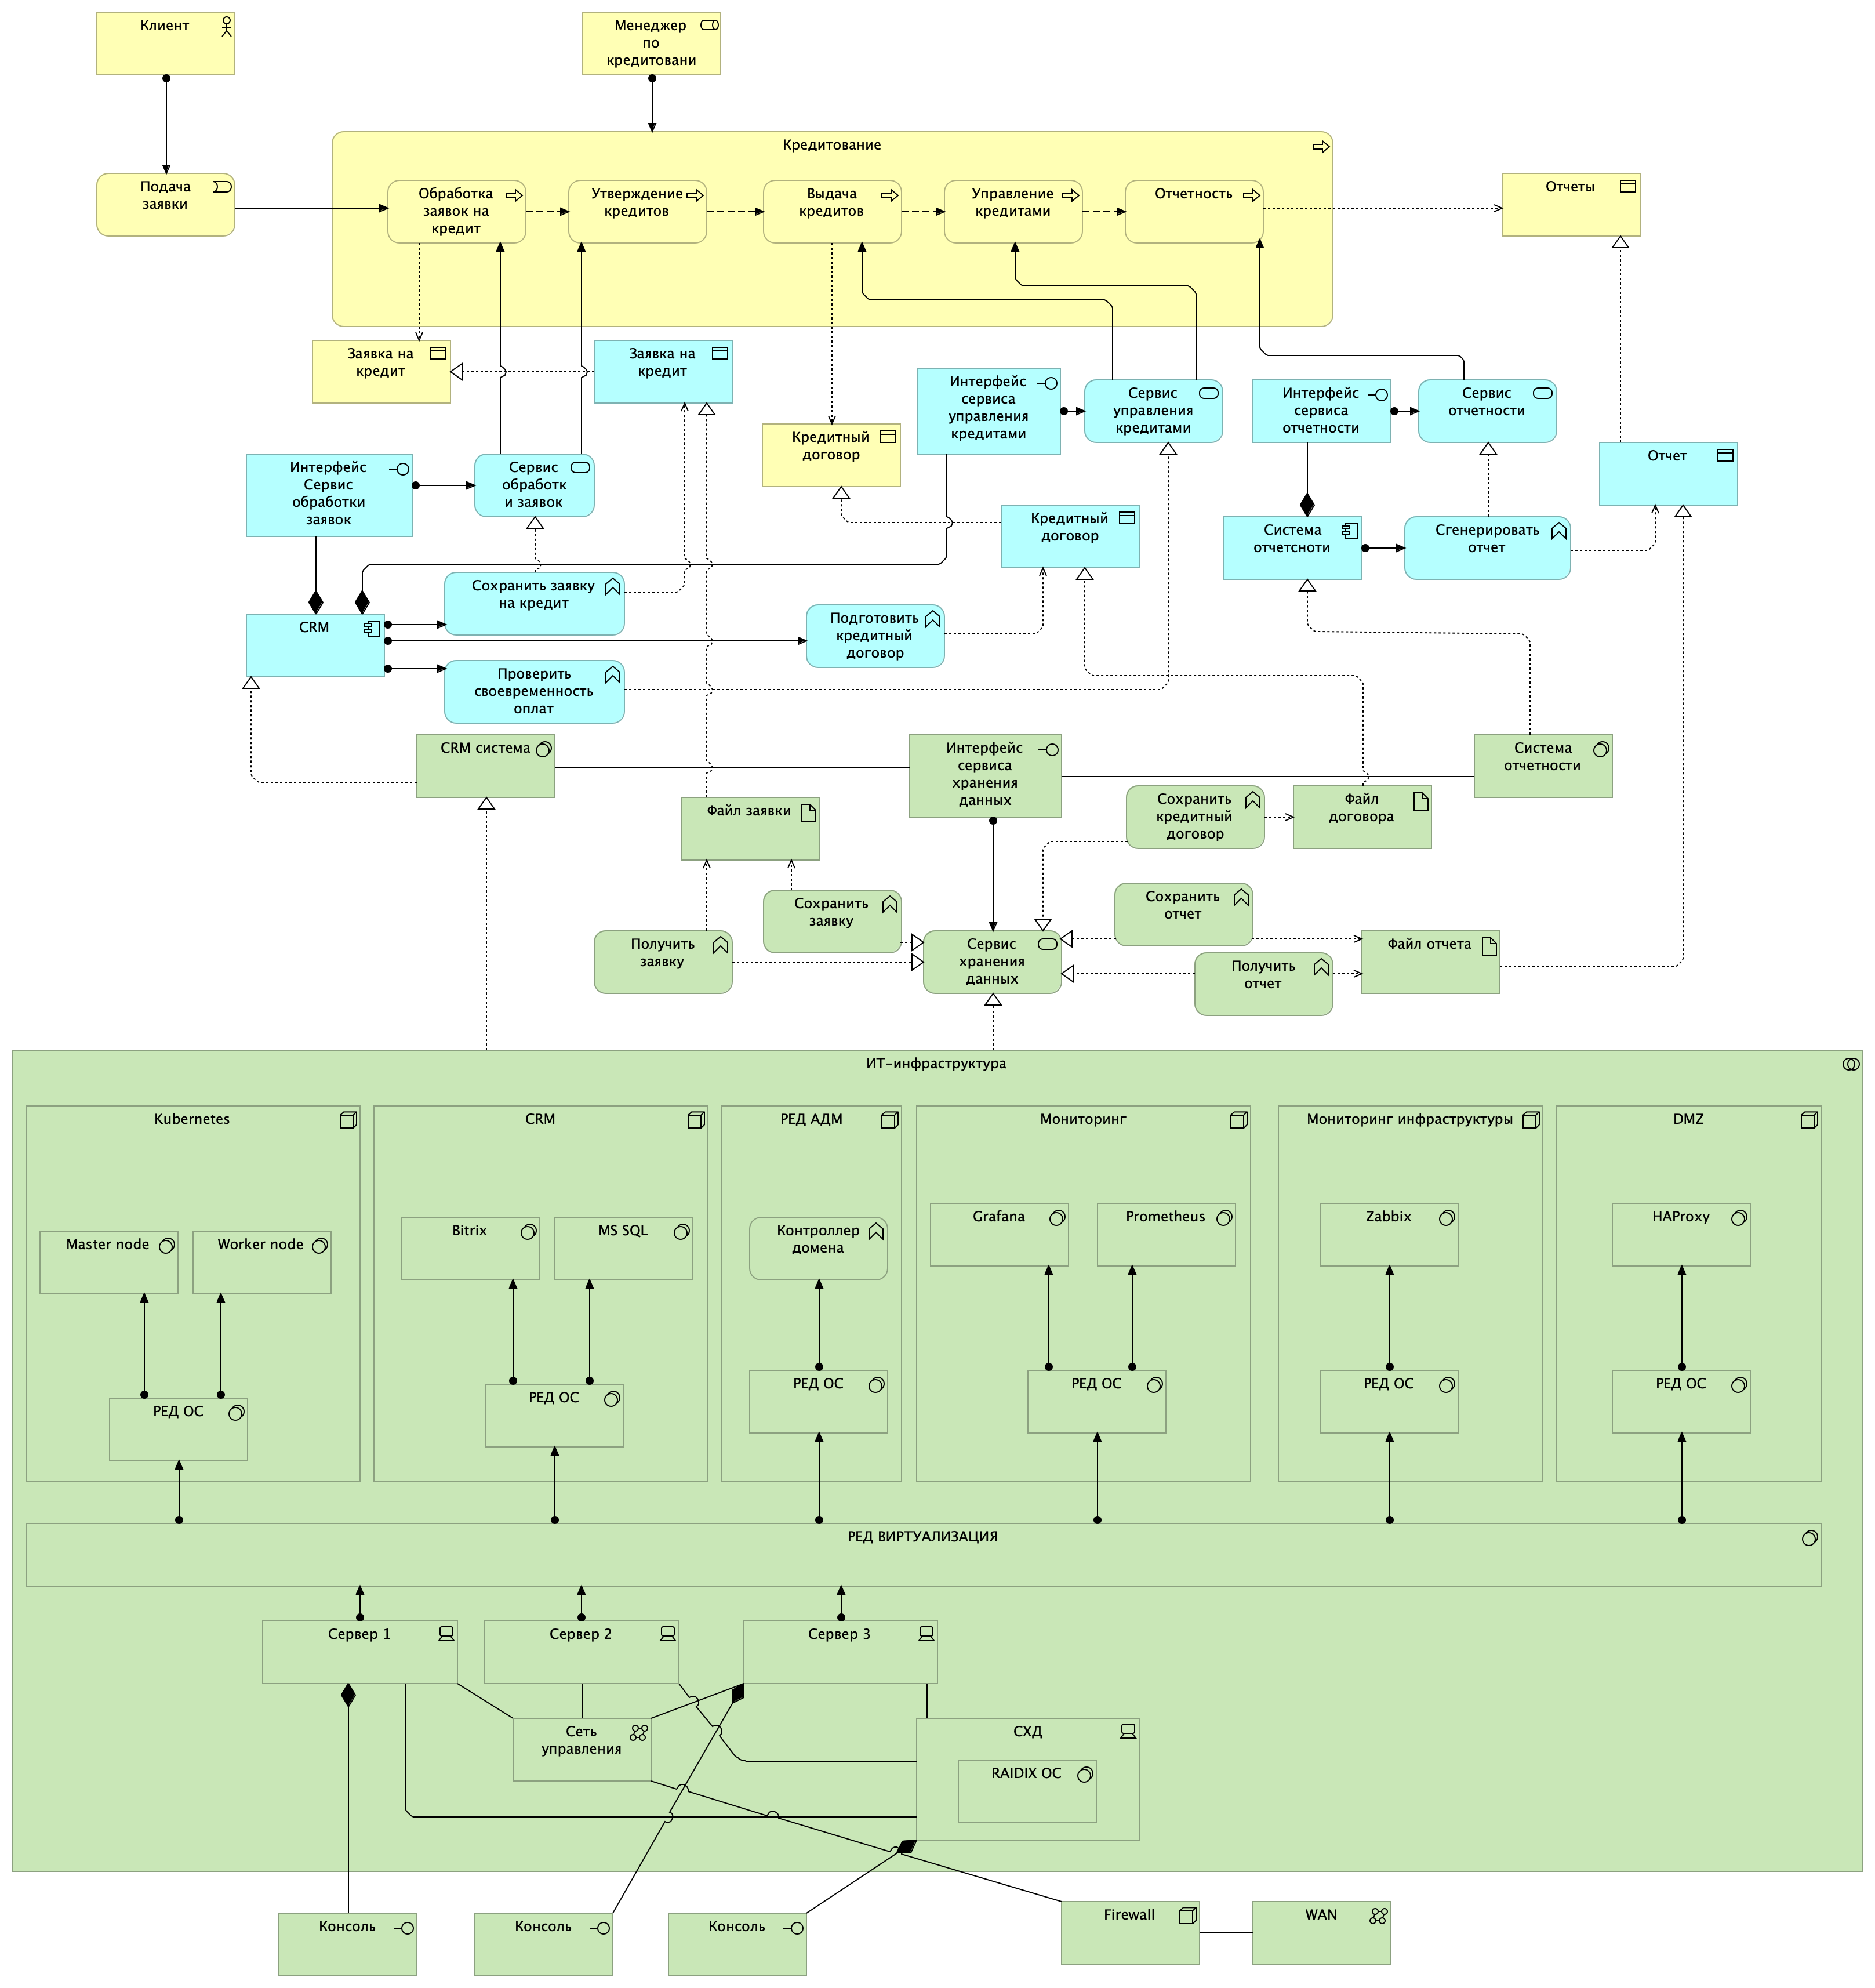
\includegraphics[width=0.9\textwidth]{archi_tobe.png}
  \caption{Диаграмма на языке ArchiMate <<to be>>}
  \label{fig:archi_tobe}
\end{figure}

\section{Заключение}
В ходе работы были рассмотрены различные варианты поставки информационно-технологического сервиса, проведен анализ компонентов инфраструктуры, выбраны системное и прикладное программное обеспечение, а также разработаны топологии развертывания и сетевой инфраструктуры. На основе проведенного анализа был обоснован выбор полностью самостоятельного варианта поставки инфраструктуры, что позволяет обеспечить высокий уровень безопасности, отказоустойчивости и соответствие требованиям регуляторов.

Проектируемая инфраструктура включает в себя серверы, системы хранения данных, сетевое оборудование и программное обеспечение, обеспечивающее выполнение ключевых бизнес-функций. Особое внимание уделено вопросам резервного копирования, аварийного восстановления и обеспечения отказоустойчивости. Использование отечественного оборудования и программного обеспечения позволяет снизить затраты на эксплуатацию и обеспечить соответствие требованиям импортозамещения.

Практическая значимость работы заключается в возможности применения разработанной ИТ-инфраструктуры для модернизации или внедрения модулей автоматизированных систем потребительского кредитования в кредитных организациях. Это способствует повышению надежности, производительности и безопасности информационных систем, а также улучшению качества обслуживания клиентов. Полученные результаты могут быть использованы в дальнейшем для масштабирования и адаптации инфраструктуры под изменяющиеся потребности бизнеса.

% used resources list
\begingroup
\let\itshape\upshape
\sloppy
\raggedright
\printbibliography[title=СПИСОК ИСПОЛЬЗУЕМЫХ ИСТОЧНИКОВ]
\phantomsection
\addcontentsline{toc}{section}{СПИСОК ИСПОЛЬЗУЕМЫХ ИСТОЧНИКОВ}
\endgroup
% used resources list

\end{document}